\documentclass[
11pt, % The default document font size, options: 10pt, 11pt, 12pt
%codirector, % Uncomment to add a codirector to the title page
]{charter}

\usepackage{tikz}
\usetikzlibrary{positioning, arrows.meta, fit, backgrounds, calc}

% ---------------------------------------------------------------------------
% REVISION QUE SE COMPILA
%   1 -> secciones 1 a 5     2 -> hasta la 9     3 -> hasta la 12    4 -> plan completo
% Las secciones aun no completadas se emiten con el texto original de la plantilla.
% Se puede sobreescribir desde la linea de comandos (ver el Makefile).
\providecommand{\revision}{1}
% ---------------------------------------------------------------------------

% Paleta pastel usada en el diagrama en bloques y en el diagrama de Gantt
\definecolor{colorOffline}{RGB}{214,234,248}
\definecolor{colorTarget}{RGB}{252,235,215}
\definecolor{colorSalida}{RGB}{226,240,217}
\definecolor{colorTecnico}{RGB}{174,208,236}
\definecolor{colorNoTecnico}{RGB}{247,209,168}
\definecolor{colorPausa}{RGB}{223,223,223}
\definecolor{colorHito}{RGB}{201,178,222}

% El títulos de la memoria, se usa en la carátula y se puede usar el cualquier lugar del documento con el comando \ttitle
\titulo{Detección de NLoS basada en IA para SoCs de UWB}

% Nombre del posgrado, se usa en la carátula y se puede usar el cualquier lugar del documento con el comando \degreename
%\posgrado{Carrera de Especialización en Sistemas Embebidos}
%\posgrado{Carrera de Especialización en Internet de las Cosas}
%\posgrado{Carrera de Especialización en Inteligencia Artificial}
%\posgrado{Maestría en Sistemas Embebidos}
%\posgrado{Maestría en Internet de las cosas}
\posgrado{Maestría en Inteligencia Artificial Embebida}

% Tu nombre, se puede usar el cualquier lugar del documento con el comando \authorname
% IMPORTANTE: no omitir titulaciones ni tildación en los nombres, también se recomienda escribir los nombres completos (tal cual los tienen en su documento)
\autor{Esp. Ing. Lautaro Vera}

% El nombre del director y co-director, se puede usar el cualquier lugar del documento con el comando \supname y \cosupname y \pertesupname y \pertecosupname
\director{\textcolor{red}{A designar}}
\pertenenciaDirector{FIUBA}
\codirector{} % para que aparezca en la portada se debe descomentar la opción codirector en los parámetros de documentclass
\pertenenciaCoDirector{FIUBA}

% Nombre del cliente, quien va a aprobar los resultados del proyecto, se puede usar con el comando \clientename y \empclientename
\cliente{Carlos Paternain}
\empresaCliente{MobileKnowledge}

\fechaINICIO{25 de agosto de 2026}		%Fecha de inicio de la cursada de GdP \fechaInicioName
\fechaFINALPlan{27 de octubre de 2026} 	%Fecha de final de cursada de GdP
\fechaFINALTrabajo{15 de noviembre de 2027}	%Fecha de defensa pública del trabajo final


\begin{document}

\maketitle
\thispagestyle{empty}
\pagebreak


\thispagestyle{empty}
{\setlength{\parskip}{0pt}
\tableofcontents{}
}
\pagebreak


\section*{Registros de cambios}
\label{sec:registro}


\begin{table}[ht]
\label{tab:registro}
\centering
\begin{tabularx}{\linewidth}{@{}|c|X|c|@{}}
\hline
\rowcolor[HTML]{C0C0C0}
Revisión & \multicolumn{1}{c|}{\cellcolor[HTML]{C0C0C0}Detalles de los cambios realizados} & Fecha      \\ \hline
0      & Creación del documento                                 &\fechaInicioName \\ \hline
\ifnum\revision>0
1      & Se completa hasta la sección 5 inclusive               & 8 de septiembre de 2026 \\ \hline
\fi
\ifnum\revision>1
2      & Se completa hasta la sección 9 inclusive               & 22 de septiembre de 2026 \\ \hline
\fi
\ifnum\revision>2
3      & Se completa hasta la sección 12 inclusive              & 6 de octubre de 2026 \\ \hline
\fi
\ifnum\revision>3
4      & Se completa el plan	                                 & \fechaFinalPlanName \\ \hline
\fi

\end{tabularx}
\end{table}

\pagebreak



\section*{Acta de constitución del proyecto}
\label{sec:acta}

\begin{flushright}
Buenos Aires, \fechaInicioName
\end{flushright}

\vspace{2cm}

Por medio de la presente se acuerda con el \authorname\hspace{1px} que su Trabajo Final de la \degreename\hspace{1px} se titulará ``\ttitle'' y consistirá en el desarrollo de un modelo de aprendizaje profundo de bajo consumo de memoria, capaz de clasificar la respuesta al impulso del canal de un enlace de banda ultra ancha como línea de visión o sin línea de visión, junto con el prototipo de firmware que ejecuta su inferencia sobre un microcontrolador Cortex-M33. El trabajo tendrá un presupuesto preliminar estimado de 600 horas y un costo estimado de \textcolor{red}{USD 15.000}, con fecha de inicio el \fechaInicioName\hspace{1px} y fecha de presentación pública el \fechaFinalName.

Se adjunta a esta acta la planificación inicial.

\vfill

% Esta parte se construye sola con la información que hayan cargado en el preámbulo del documento y no debe modificarla
\begin{table}[ht]
\centering
\begin{tabular}{ccc}
\begin{tabular}[c]{@{}c@{}}Dr. Ing. Ariel Lutenberg \\ Director posgrado FIUBA\end{tabular} & \hspace{2cm} & \begin{tabular}[c]{@{}c@{}}\clientename \\ \empclientename \end{tabular} \vspace{2.5cm} \\
\multicolumn{3}{c}{\begin{tabular}[c]{@{}c@{}} \supname \\ Director del Trabajo Final\end{tabular}} \vspace{2.5cm} \\
\end{tabular}
\end{table}




\section{1. Descripción técnica-conceptual del proyecto a realizar}
\label{sec:descripcion}

Los transceptores de banda ultra ancha (UWB, por \textit{ultra-wideband}) permiten medir distancias con una precisión del orden del centímetro y sostienen buena parte de los sistemas de localización en tiempo real (RTLS) que se despliegan hoy en logística, control de acceso y llave digital vehicular. Esa precisión se degrada de manera significativa cuando el trayecto directo entre los dos dispositivos se encuentra obstruido, condición conocida como ausencia de línea de visión (NLoS, por \textit{non-line-of-sight}). En esa situación el receptor identifica como primer camino una réplica reflejada de la señal y la distancia estimada resulta mayor que la real, con errores que pueden alcanzar varios decímetros. La detección confiable de la condición NLoS es, por lo tanto, la principal palanca disponible para mejorar la exactitud del \textit{ranging}.

En los productos actuales esa detección se resuelve mediante algoritmos de procesamiento digital de señales integrados en el propio chip, que aplican reglas deterministas sobre un conjunto reducido de métricas de canal, como la amplitud del primer camino o la potencia total recibida. El enfoque tiene la ventaja del determinismo y del bajo consumo, pero descarta la mayor parte de la información contenida en la respuesta al impulso del canal (CIR, por \textit{channel impulse response}). En paralelo, la literatura reciente muestra que los modelos de aprendizaje profundo aplicados sobre la CIR completa alcanzan tasas de acierto muy superiores. Esos trabajos, entre ellos la arquitectura ADCNN-BiLSTM-Transformer publicada en \textit{IEEE Journals}, se ejecutan fuera del chip, sobre un procesador de propósito general, porque su tamaño excede ampliamente la memoria disponible en un transceptor UWB.

El proyecto se ubica en ese espacio intermedio. Se propone desarrollar un modelo convolucional unidimensional de bajo perfil en memoria, cuantizado a enteros de 8 bits, que clasifique la CIR como LoS o NLoS con una exactitud comparable a la de los modelos publicados, pero con un tamaño compatible con la memoria de un dispositivo embebido. El entregable es un producto mínimo viable que demuestra la factibilidad de trasladar la inferencia al borde, como paso previo a su integración en un transceptor comercial de la familia NXP SR250 o NCJ29D6.

El contexto es empresarial. El trabajo se realiza en MobileKnowledge, compañía especializada en tecnologías de conectividad de corto alcance y socia tecnológica de NXP Semiconductors. La empresa aporta el conocimiento de dominio en UWB y el acceso al hardware de evaluación. El proyecto no cuenta con financiamiento público ni privado específico. El material técnico provisto por NXP se encuentra alcanzado por un acuerdo de confidencialidad, por lo que no se reproducen fragmentos de su documentación ni de su código en los entregables.

La propuesta de valor se apoya en tres puntos. Primero, la solución opera sobre datos que el transceptor ya calcula, sin necesidad de sensores adicionales ni de cambios en el protocolo de \textit{ranging}. Segundo, al ejecutarse en el dispositivo elimina la latencia y el consumo asociados a enviar la CIR completa a un procesador externo, que en el caso de una CIR de 1016 muestras representa un volumen de datos considerable para un enlace embebido. Tercero, el modelo se diseña desde el inicio con un presupuesto de memoria explícito, criterio ausente en los trabajos académicos de referencia, que priorizan la exactitud sin restricciones de plataforma.

En la figura \ref{fig:diagBloques} se presenta el diagrama en bloques del sistema. Se observan dos cadenas de procesamiento. La cadena superior corresponde al entorno de desarrollo, donde el conjunto de datos público se prepara, se emplea para entrenar la red convolucional, y el modelo resultante se cuantiza y se convierte en un arreglo de C que se enlaza con el firmware. La cadena inferior corresponde al sistema embebido: el transceptor UWB entrega la CIR de cada intercambio de \textit{ranging}, el firmware la acondiciona, el motor de inferencia produce la decisión entre LoS y NLoS, y esa decisión se utiliza para ponderar o descartar la medición de distancia antes de entregarla a la aplicación de localización.

\begin{figure}[htpb]
\centering
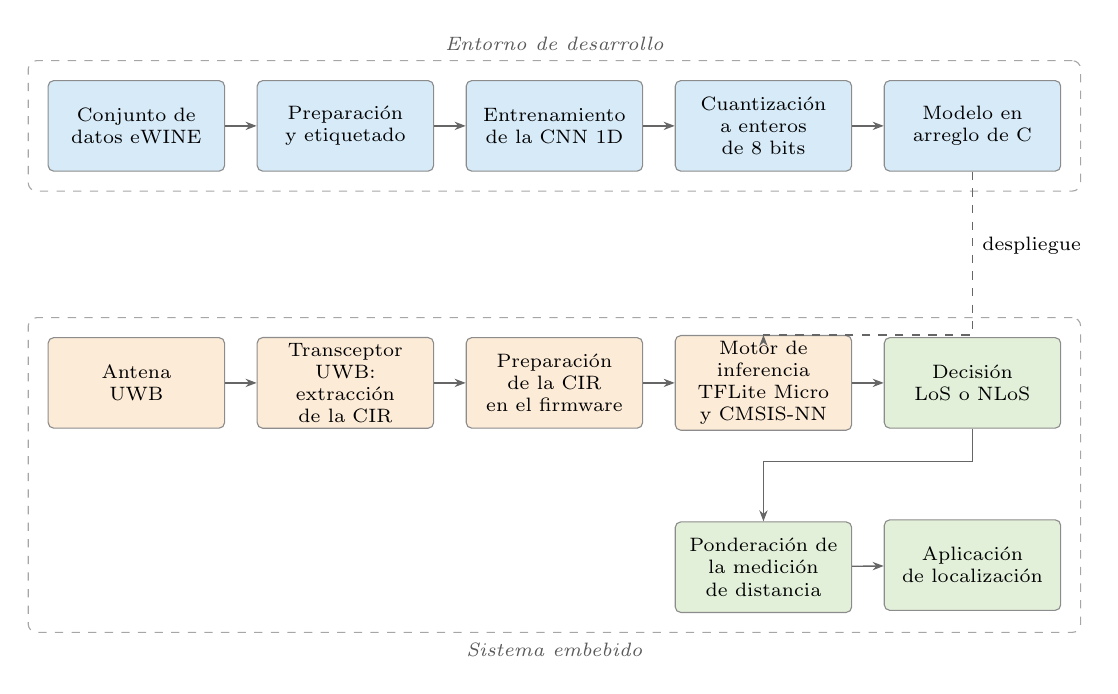
\begin{tikzpicture}[
	font=\scriptsize,
	bloque/.style={rectangle, rounded corners=2pt, draw=black!45, line width=0.4pt,
	               align=center, text width=2.1cm, minimum height=1.15cm, inner sep=2pt},
	offline/.style={bloque, fill=colorOffline},
	target/.style={bloque, fill=colorTarget},
	salida/.style={bloque, fill=colorSalida},
	flecha/.style={-{Stealth[length=4pt]}, draw=black!60, line width=0.5pt},
	]

% Cadena de desarrollo
\node[offline] (a1) {Conjunto de\\datos eWINE};
\node[offline, right=0.4cm of a1] (a2) {Preparación\\y etiquetado};
\node[offline, right=0.4cm of a2] (a3) {Entrenamiento\\de la CNN 1D};
\node[offline, right=0.4cm of a3] (a4) {Cuantización\\a enteros\\de 8 bits};
\node[offline, right=0.4cm of a4] (a5) {Modelo en\\arreglo de C};

\draw[flecha] (a1) -- (a2);
\draw[flecha] (a2) -- (a3);
\draw[flecha] (a3) -- (a4);
\draw[flecha] (a4) -- (a5);

% Cadena embebida
\node[target, below=2.1cm of a1] (b1) {Antena\\UWB};
\node[target, right=0.4cm of b1] (b2) {Transceptor\\UWB:\\extracción\\de la CIR};
\node[target, right=0.4cm of b2] (b3) {Preparación\\de la CIR\\en el firmware};
\node[target, right=0.4cm of b3] (b4) {Motor de inferencia\\TFLite Micro\\y CMSIS-NN};
\node[salida, right=0.4cm of b4] (b5) {Decisión\\LoS o NLoS};

\draw[flecha] (b1) -- (b2);
\draw[flecha] (b2) -- (b3);
\draw[flecha] (b3) -- (b4);
\draw[flecha] (b4) -- (b5);

\node[salida, below=1.15cm of b4] (c1) {Ponderación de\\la medición\\de distancia};
\node[salida, below=1.15cm of b5] (c2) {Aplicación\\de localización};

\draw[flecha] (b5.south) -- ++(0,-0.42) -| (c1.north);
\draw[flecha] (c1) -- (c2);

% Despliegue del modelo entrenado sobre el sistema embebido
\draw[flecha, dashed] (a5.south) -- node[right, pos=0.45, font=\scriptsize] {despliegue} (a5.south|-b4.north) -| (b4.north);

\begin{scope}[on background layer]
	\node[draw=black!35, dashed, rounded corners=3pt, inner sep=7pt,
	      fit=(a1)(a5), label={[font=\scriptsize\itshape, black!65]above:Entorno de desarrollo}] (grupoA) {};
	\node[draw=black!35, dashed, rounded corners=3pt, inner sep=7pt,
	      fit=(b1)(b5)(c1)(c2), label={[font=\scriptsize\itshape, black!65]below:Sistema embebido}] (grupoB) {};
\end{scope}

\end{tikzpicture}
\caption{Diagrama en bloques del sistema.}
\label{fig:diagBloques}
\end{figure}

Los bloques de la cadena de desarrollo se ejecutan una sola vez, durante el proyecto, sobre una computadora personal. Los bloques de la cadena embebida se ejecutan en cada intercambio de \textit{ranging} y son los que imponen las restricciones de memoria y de tiempo de respuesta que condicionan el diseño del modelo. El bloque de preparación de la CIR resuelve la alineación de la CIR respecto del primer camino detectado y su normalización, y es la pieza que garantiza que el modelo reciba una entrada equivalente a la que se usó durante el entrenamiento.

En términos de ciclo de vida, la solución se encuentra en etapa de prueba de concepto. El proyecto la lleva hasta un prototipo validado sobre hardware de evaluación, con métricas de exactitud, memoria y latencia medidas. La integración en un producto comercial queda fuera del alcance y depende de decisiones posteriores de la empresa y de su socio tecnológico.

\section{2. Identificación y análisis de los interesados}
\label{sec:interesados}

En la tabla \ref{tab:interesados} se identifican los interesados del proyecto y el rol que ocupa cada uno.

\begin{table}[ht]
\caption{Identificación de los interesados.}
\label{tab:interesados}
\begin{tabularx}{\linewidth}{@{}|l|X|X|l|@{}}
\hline
\rowcolor[HTML]{C0C0C0}
Rol           & Nombre y Apellido & Organización 	& Puesto 	\\ \hline
Cliente       & \clientename      &\empclientename	& Responsable técnico \\ \hline
Responsable   & \authorname       & FIUBA        	& Alumno 	\\ \hline
Orientador    & \supname	      & \pertesupname 	& Director del Trabajo Final \\ \hline
Colaboradores & Equipo de ingeniería UWB & \empclientename & Ingenieros de aplicación \\ \hline
Usuario final & Integradores de sistemas RTLS y desarrolladores de firmware UWB & Empresas del sector & - \\ \hline
\end{tabularx}
\end{table}

A continuación se describen las características de cada interesado que resultan relevantes para la planificación.

\begin{itemize}
	\item Cliente: Carlos Paternain aprueba los entregables y participa en la definición de los criterios de aceptación. Conoce en profundidad la tecnología UWB y las limitaciones de los transceptores de NXP, por lo que su revisión es determinante para validar que el presupuesto de memoria adoptado sea realista. Su disponibilidad se concentra fuera de los períodos de lanzamiento de producto, de modo que las revisiones se acuerdan con antelación.
	\item Responsable: el alumno ejecuta la totalidad de las tareas técnicas y de documentación. Cursa el posgrado en paralelo con su actividad profesional, condición que fija la dedicación semanal disponible y que se refleja en el cronograma.
	\item Orientador: el director del Trabajo Final orienta las decisiones metodológicas, en particular el diseño de la validación y la interpretación de las métricas. Se prevén encuentros de seguimiento al cierre de cada bloque de sprints.
	\item Colaboradores: el equipo de ingeniería UWB de MobileKnowledge facilita el acceso al hardware de evaluación y responde consultas sobre el formato de la CIR. Su participación es puntual y no se le asignan tareas del cronograma.
	\item Usuario final: los integradores de sistemas RTLS y los desarrolladores de firmware UWB son quienes adoptarían la solución. Valoran la exactitud del \textit{ranging}, el consumo de memoria y la ausencia de cambios en el protocolo existente.
\end{itemize}

\section{3. Propósito del proyecto}
\label{sec:proposito}

El propósito de este proyecto es demostrar que la detección de la condición sin línea de visión en enlaces de banda ultra ancha puede resolverse con un modelo de aprendizaje profundo lo suficientemente pequeño como para ejecutarse dentro de un dispositivo embebido, y no solo en un procesador externo, de manera de mejorar la exactitud de la medición de distancia sin agregar hardware, sin modificar el protocolo de \textit{ranging} y sin transferir la respuesta al impulso del canal fuera del dispositivo.

\section{4. Alcance del proyecto}
\label{sec:alcance}

El proyecto incluye:

\begin{itemize}
	\item La construcción de un flujo reproducible de ingesta del conjunto de datos público eWINE, con particiones versionadas para entrenamiento, validación y prueba.
	\item El análisis exploratorio de las respuestas al impulso del canal, discriminado por clase y por entorno de medición, y la documentación de los sesgos detectados.
	\item El diseño e implementación del preprocesamiento de la CIR, que comprende:
		\begin{itemize}
		\item La alineación respecto del primer camino detectado.
		\item La normalización de amplitud.
		\item La selección del ancho de ventana que minimiza el uso de memoria sin degradar la exactitud.
		\end{itemize}
	\item El entrenamiento de una red convolucional unidimensional de referencia y de dos modelos de comparación clásicos sobre las métricas de canal.
	\item La exploración de arquitecturas sujeta a un presupuesto de memoria explícito, con poda estructurada del modelo seleccionado.
	\item La cuantización del modelo a enteros de 8 bits y la verificación de compatibilidad con el conjunto de operadores de TensorFlow Lite for Microcontrollers.
	\item El desarrollo del firmware de prueba que ejecuta la inferencia sobre un microcontrolador Cortex-M33 con aceleración CMSIS-NN.
	\item La medición sobre el hardware de evaluación de la memoria de programa ocupada, la memoria de trabajo del intérprete, la latencia de inferencia y la exactitud alcanzada.
	\item La comparación de los resultados del modelo contra el criterio determinista de referencia disponible en el transceptor.
	\item La elaboración del informe de avance y de la memoria técnica.
\end{itemize}

El presente proyecto no incluye:

\begin{itemize}
	\item La realización de campañas de medición propias para generar un conjunto de datos nuevo.
	\item La integración del modelo dentro del firmware productivo de los transceptores SR250 o NCJ29D6, ni la modificación de su código propietario.
	\item El desarrollo de una aplicación de localización en tiempo real completa.
	\item Los ensayos de certificación de espectro radioeléctrico y de compatibilidad electromagnética.
	\item La industrialización, la fabricación de hardware a medida y cualquier actividad de puesta en el mercado.
	\item La detección o corrección del error de \textit{ranging} en magnitud, que constituye un problema de regresión distinto del problema de clasificación abordado.
\end{itemize}

\section{5. Supuestos del proyecto}
\label{sec:supuestos}

Para el desarrollo del presente proyecto se supone que:

\begin{itemize}
	\item El alumno dispone de al menos 16 horas semanales durante los períodos activos del cronograma, y de las condiciones de salud necesarias para sostener esa dedicación.
	\item MobileKnowledge mantiene el interés en el proyecto y la asignación del cliente durante todo el período, sin que un cambio de prioridades comerciales interrumpa las instancias de revisión.
	\item La empresa provee una placa de evaluación con microcontrolador Cortex-M33 y su cadena de compilación durante toda la etapa de despliegue.
	\item El conjunto de datos eWINE permanece disponible en su repositorio público y sus condiciones de uso no se modifican de manera restrictiva.
	\item La respuesta al impulso del canal contiene información suficiente para discriminar las condiciones LoS y NLoS con la exactitud objetivo, tal como reportan los trabajos publicados sobre el mismo conjunto de datos.
	\item Las herramientas de código abierto empleadas, entre ellas TensorFlow, TensorFlow Lite for Microcontrollers y CMSIS-NN, conservan sus licencias permisivas actuales.
	\item El equipamiento de cómputo disponible resulta suficiente para entrenar los modelos previstos, cuyo tamaño es reducido, sin necesidad de contratar infraestructura en la nube.
\end{itemize}

\ifnum\revision>1
\section{6. Product Backlog}
\label{sec:backlog}

El Product Backlog se organiza en cuatro épicas que se corresponden con los bloques funcionales del sistema descrito en la sección \ref{sec:descripcion}: la obtención y comprensión de los datos, su preparación, el modelado y su optimización, y el despliegue sobre el sistema embebido.

\textbf{Criterio de cálculo de los Story Points.} Cada historia de usuario se puntúa en tres dimensiones, con valores enteros de 1 a 5:

\begin{itemize}
	\item Dificultad (D): cantidad de trabajo involucrado.
	\item Complejidad (C): nivel técnico o sofisticación de la solución.
	\item Incertidumbre (I): nivel de riesgo o de novedad respecto de la experiencia previa.
\end{itemize}

La suma de las tres dimensiones se redondea al valor superior más cercano de la serie de Fibonacci (1, 2, 3, 5, 8, 13, 21, 34). Por ejemplo, una historia que suma 12 puntos recibe 13 Story Points. Los Story Points expresan el tamaño relativo de una historia frente a las demás y no se equiparan con horas de trabajo.

\subsection{Épica 1: ingesta y comprensión de los datos}

\begin{itemize}
	\item \textbf{HU1.} Como desarrollador de modelos, quiero disponer de un flujo reproducible que convierta el conjunto de datos eWINE en tensores de CIR etiquetados, para entrenar modelos sin repetir el trabajo de preparación en cada experimento. Prioridad alta.
	\item \textbf{HU2.} Como desarrollador de modelos, quiero un análisis exploratorio de las CIR discriminado por clase y por entorno, para identificar sesgos de distribución y definir un esquema de partición que permita medir la generalización. Prioridad alta.
\end{itemize}

\subsection{Épica 2: preprocesamiento y representación de la CIR}

\begin{itemize}
	\item \textbf{HU3.} Como desarrollador de modelos, quiero alinear cada CIR respecto de su primer camino detectado y normalizar su amplitud, para que el modelo aprenda la forma del perfil de multitrayecto y no la posición absoluta de la ventana de captura. Prioridad alta.
	\item \textbf{HU4.} Como desarrollador de modelos, quiero reducir la ventana de CIR al menor número de muestras que preserve la exactitud, para acotar la memoria de trabajo que el modelo requiere en el dispositivo. Prioridad alta.
\end{itemize}

\subsection{Épica 3: modelado y optimización para el sistema embebido}

\begin{itemize}
	\item \textbf{HU5.} Como desarrollador de modelos, quiero entrenar una red convolucional unidimensional sobre las CIR preprocesadas, para obtener una línea base de clasificación entre LoS y NLoS contra la cual comparar las variantes posteriores. Prioridad alta.
	\item \textbf{HU6.} Como desarrollador de modelos, quiero explorar variantes de arquitectura sujetas a un presupuesto de memoria explícito, para elegir el mejor compromiso entre exactitud y tamaño del modelo. Prioridad alta.
	\item \textbf{HU7.} Como desarrollador de firmware, quiero cuantizar el modelo seleccionado a enteros de 8 bits, para reducir su ocupación en memoria de programa y habilitar la ejecución acelerada con CMSIS-NN. Prioridad alta.
\end{itemize}

\subsection{Épica 4: despliegue y validación sobre el sistema embebido}

\begin{itemize}
	\item \textbf{HU8.} Como desarrollador de firmware, quiero ejecutar el modelo cuantizado sobre el microcontrolador Cortex-M33, para verificar que la inferencia entra en la memoria disponible y responde dentro del tiempo requerido. Prioridad alta.
	\item \textbf{HU9.} Como desarrollador de firmware, quiero medir y comparar la memoria ocupada, la latencia y la exactitud entre la computadora personal y el dispositivo, para demostrar que la degradación introducida por la cuantización se mantiene acotada. Prioridad alta.
	\item \textbf{HU10.} Como responsable técnico del producto, quiero comparar el detector basado en aprendizaje profundo contra el criterio determinista de referencia, para cuantificar la mejora que aporta la solución propuesta. Prioridad media. Historia opcional.
\end{itemize}

En la tabla \ref{tab:storypoints} se presenta la ponderación de cada historia de usuario.

\begin{table}[htpb]
\centering
\caption{Ponderación de las historias de usuario en Story Points.}
\label{tab:storypoints}
\begin{tabularx}{\linewidth}{@{}|c|X|c|c|c|c|c|c|@{}}
\hline
\rowcolor[HTML]{C0C0C0}
HU & Épica & D & C & I & Suma & SP & Prioridad \\ \hline
HU1 & Ingesta y comprensión de los datos & 2 & 2 & 1 & 5 & 5 & Alta \\ \hline
HU2 & Ingesta y comprensión de los datos & 2 & 1 & 1 & 4 & 5 & Alta \\ \hline
HU3 & Preprocesamiento y representación & 3 & 3 & 2 & 8 & 8 & Alta \\ \hline
HU4 & Preprocesamiento y representación & 3 & 2 & 2 & 7 & 8 & Alta \\ \hline
HU5 & Modelado y optimización & 3 & 3 & 2 & 8 & 8 & Alta \\ \hline
HU6 & Modelado y optimización & 4 & 4 & 4 & 12 & 13 & Alta \\ \hline
HU7 & Modelado y optimización & 3 & 4 & 4 & 11 & 13 & Alta \\ \hline
HU8 & Despliegue y validación & 4 & 4 & 5 & 13 & 13 & Alta \\ \hline
HU9 & Despliegue y validación & 3 & 2 & 2 & 7 & 8 & Alta \\ \hline
HU10 & Despliegue y validación & 2 & 3 & 3 & 8 & 8 & Media (opcional) \\ \hline
\rowcolor[HTML]{EFEFEF}
\multicolumn{6}{|r|}{Total} & 89 & \\ \hline
\end{tabularx}
\end{table}
\else\section{6. Product Backlog}
\label{sec:backlog}


\begin{consigna}{red}
El Product Backlog debe organizarse en cuatro \textbf{\textit{\'{e}picas}} fundamentales del proyecto. Cada \'{e}pica debe contener al menos dos historias de usuario que describan funcionalidades clave.

El Product Backlog debe permitir interpretar cómo será el proyecto y su funcionalidad. Se deben indicar claramente las prioridades entre las historias de usuario y si hay alguna opcional.

Las historias de usuario deben ser breves, claras y medibles, expresando el rol, la necesidad y el propósito de cada funcionalidad. También deben tener una prioridad definida para facilitar la planificación de los sprints.

Cada historia de usuario debe incluir una ponderación en \textit{Story Points}, un número entero que representa el tama\~no relativo de la historia. El criterio para calcular los Story Points debe indicarse explícitamente.

Las historias deben seguir el formato: ``\textit{Como [rol], quiero [tal cosa] para [tal otra cosa]}''.

Las \'{e}picas deben estructurarse de la siguiente forma:

\begin{itemize}
  \item \textbf{\'{E}pica 1}
    \begin{itemize}
      \item HU1
      \item HU2
    \end{itemize}
  \item \textbf{\'{E}pica 2}
    \begin{itemize}
      \item HU3
      \item HU4
    \end{itemize}
  \item \textbf{\'{E}pica 3}
    \begin{itemize}
      \item HU5
      \item HU6
    \end{itemize}
  \item \textbf{\'{E}pica 4}
    \begin{itemize}
      \item HU7
      \item HU8
    \end{itemize}
\end{itemize}

\textbf{Reglas para definir historias de usuario:}
\begin{itemize}
  \item Ser concisas y claras.
  \item Expresarlas en términos cuantificables y medibles.
  \item No dejar margen para interpretaciones ambiguas.
  \item Indicar claramente su prioridad y si son opcionales.
  \item Considerar regulaciones y normas vigentes.
\end{itemize}
\end{consigna}
\fi

\ifnum\revision>1
\section{7. Criterios de aceptación de historias de usuario}
\label{sec:criteriosAceptacion}

\subsection{Épica 1: ingesta y comprensión de los datos}

\textbf{Criterios de aceptación de HU1}
\begin{itemize}
	\item El flujo procesa las 42.000 muestras del conjunto de datos y finaliza en menos de 5 minutos sobre la computadora de desarrollo.
	\item Dos ejecuciones con la misma semilla producen particiones de entrenamiento, validación y prueba idénticas, verificadas por la suma de verificación de los índices.
	\item El conjunto de prueba conserva la proporción entre las clases LoS y NLoS del conjunto original con una diferencia no mayor a 1 punto porcentual.
	\item El flujo aborta con un mensaje explícito si alguno de los siete subconjuntos de origen falta o presenta un número de columnas distinto del esperado.
\end{itemize}

\textbf{Criterios de aceptación de HU2}
\begin{itemize}
	\item El informe de análisis presenta, para cada uno de los siete entornos, el número de muestras por clase y las estadísticas descriptivas de las métricas de canal.
	\item El informe incluye la CIR promedio y las bandas de percentiles 10 y 90 para cada clase y cada entorno.
	\item El informe cuantifica el desbalance entre entornos y enuncia de manera explícita los sesgos detectados y su efecto previsible sobre la generalización.
	\item El informe se regenera de manera automática a partir del flujo de datos, sin pasos manuales.
\end{itemize}

\subsection{Épica 2: preprocesamiento y representación de la CIR}

\textbf{Criterios de aceptación de HU3}
\begin{itemize}
	\item El módulo de alineación ubica el primer camino en la misma posición de la ventana para el 100 \% de las muestras procesadas.
	\item Cada CIR normalizada presenta energía unitaria, verificado con una tolerancia relativa de $10^{-6}$.
	\item Se documenta la comparación de exactitud entre al menos dos esquemas de normalización sobre un clasificador de referencia, con la misma partición y la misma semilla.
	\item El preprocesamiento se expresa como una transformación encadenable, aplicable de manera idéntica en entrenamiento y en inferencia.
\end{itemize}

\textbf{Criterios de aceptación de HU4}
\begin{itemize}
	\item Se ejecuta un barrido de anchos de ventana con al menos cuatro valores comprendidos entre 32 y 256 muestras.
	\item Para cada ancho se registra la exactitud de validación y la memoria de trabajo requerida, expresada en bytes.
	\item El ancho seleccionado no reduce la exactitud de validación en más de 1 punto porcentual respecto del mejor valor del barrido.
	\item La decisión adoptada queda documentada junto con la curva de compromiso entre exactitud y memoria.
\end{itemize}

\subsection{Épica 3: modelado y optimización para el sistema embebido}

\textbf{Criterios de aceptación de HU5}
\begin{itemize}
	\item La red convolucional alcanza un valor de F1 igual o superior a 0,90 sobre el conjunto de prueba con partición estratificada.
	\item Se reportan exactitud, precisión, exhaustividad, F1, área bajo la curva ROC y matriz de confusión.
	\item La red supera en al menos 5 puntos de F1 a los dos modelos de comparación entrenados sobre las métricas de canal.
	\item Los resultados se reproducen a partir del registro de experimentos, que conserva la configuración, la semilla y los pesos de cada corrida.
\end{itemize}

\textbf{Criterios de aceptación de HU6}
\begin{itemize}
	\item La búsqueda evalúa al menos doce configuraciones con distinta profundidad, número de filtros y tamaño de núcleo.
	\item Toda configuración evaluada respeta el presupuesto de memoria fijado, y las que lo exceden se descartan de manera automática antes de entrenarse.
	\item Se construye la frontera de compromiso entre exactitud y tamaño del modelo, y la arquitectura elegida se justifica sobre esa frontera.
	\item El modelo podado conserva un valor de F1 que no cae más de 1 punto porcentual respecto del modelo denso equivalente.
\end{itemize}

\textbf{Criterios de aceptación de HU7}
\begin{itemize}
	\item El modelo cuantizado ocupa 64 kB de memoria de programa o menos.
	\item La caída de F1 del modelo cuantizado respecto del modelo en punto flotante no supera los 2 puntos porcentuales sobre el conjunto de prueba.
	\item La totalidad de los operadores del grafo cuantizado pertenece al conjunto de operadores soportados por TensorFlow Lite for Microcontrollers, verificado con la herramienta de inspección del grafo.
	\item El procedimiento de cuantización queda documentado, incluida la composición del conjunto representativo utilizado para la calibración.
\end{itemize}

\subsection{Épica 4: despliegue y validación sobre el sistema embebido}

\textbf{Criterios de aceptación de HU8}
\begin{itemize}
	\item El firmware compila sin advertencias y se graba en la placa de evaluación siguiendo el procedimiento documentado.
	\item La memoria de trabajo del intérprete se dimensiona de manera explícita y el firmware informa por consola el valor efectivamente utilizado.
	\item El banco de pruebas inyecta al menos 100 CIR almacenadas y devuelve la clase inferida por cada una a través del puerto serie.
	\item El firmware ejecuta 1000 inferencias consecutivas sin reinicios ni desbordamientos de pila.
\end{itemize}

\textbf{Criterios de aceptación de HU9}
\begin{itemize}
	\item Se reportan la memoria de programa y la memoria de trabajo ocupadas, obtenidas del mapa de memoria del enlazador.
	\item Se reporta la latencia de inferencia como mediana y percentil 95 sobre al menos 1000 repeticiones, medida con el contador de ciclos del procesador.
	\item La latencia mediana resulta igual o menor a 10 ms.
	\item La clase inferida en el dispositivo coincide con la inferida en la computadora personal en al menos el 99 \% de las muestras del conjunto de prueba, y las discrepancias quedan analizadas.
\end{itemize}

\textbf{Criterios de aceptación de HU10}
\begin{itemize}
	\item Se obtiene el indicador determinista de referencia para la totalidad del conjunto de prueba.
	\item Se presentan las matrices de confusión y las curvas ROC de ambos criterios sobre el mismo conjunto de prueba.
	\item La comparación se acompaña de un intervalo de confianza del 95 \% para la diferencia de F1 entre ambos criterios.
	\item Las conclusiones distinguen de manera explícita los casos en los que el criterio determinista resulta preferible.
\end{itemize}
\else\section{7. Criterios de aceptación de historias de usuario}
\label{sec:criteriosAceptacion}


\begin{consigna}{red}
Los criterios de aceptación deben establecerse para cada historia de usuario, asegurando que se cumplan las condiciones necesarias para que la funcionalidad sea validada correctamente.

Cada historia debe tener criterios medibles, específicos y verificables. Deben permitir validar que se cumple con las necesidades del usuario.

Se estructuran de forma análoga a las \'{e}picas del backlog:

\begin{itemize}
  \item \textbf{\'{E}pica 1}
    \begin{itemize}
      \item Criterios de aceptación HU1
      \item Criterios de aceptación HU2
    \end{itemize}
  \item \textbf{\'{E}pica 2}
    \begin{itemize}
      \item Criterios de aceptación HU3
      \item Criterios de aceptación HU4
    \end{itemize}
  \item \textbf{\'{E}pica 3}
    \begin{itemize}
      \item Criterios de aceptación HU5
      \item Criterios de aceptación HU6
    \end{itemize}
  \item \textbf{\'{E}pica 4}
    \begin{itemize}
      \item Criterios de aceptación HU7
      \item Criterios de aceptación HU8
    \end{itemize}
\end{itemize}

\textbf{Reglas para definir criterios de aceptación:}
\begin{itemize}
  \item Medibles y verificables.
  \item Especificar cuándo una historia se considera completada.
  \item Incluir condiciones específicas.
  \item No ambiguos.
  \item Probables de testear funcional o técnicamente.
  \item Mínimo 3 criterios por HU.
\end{itemize}
\end{consigna}
\fi

\ifnum\revision>1
\section{8. Fases de CRISP-DM}
\label{sec:crispdm}

\subsection{Comprensión del negocio}

El objetivo es aumentar la exactitud de la medición de distancia en enlaces UWB mediante la identificación confiable de la condición sin línea de visión, resuelta con un modelo de aprendizaje profundo que se ejecuta dentro del dispositivo. El impacto esperado es doble: por un lado, la reducción del error de \textit{ranging} en escenarios de interior con obstrucciones, que son los más frecuentes en aplicaciones de logística y control de acceso; por el otro, la posibilidad de descartar mediciones poco confiables antes de que contaminen el cálculo de posición.

Se adoptan tres métricas de éxito conjuntas, que deben cumplirse de manera simultánea:

\begin{itemize}
	\item Un valor de F1 igual o superior a 0,90 en la clasificación entre LoS y NLoS sobre el conjunto de prueba.
	\item Una ocupación de memoria de programa igual o menor a 64 kB para el modelo cuantizado.
	\item Una latencia de inferencia mediana igual o menor a 10 ms sobre el microcontrolador Cortex-M33.
\end{itemize}

\subsection{Comprensión de los datos}

Se trabaja con datos tabulares que contienen una señal unidimensional por registro. La fuente es el conjunto de datos público del proyecto eWINE, que reúne trazas capturadas con transceptores UWB en siete ubicaciones de interior distintas. El conjunto contiene aproximadamente 42.000 registros, balanceados entre las dos clases, con unos 21.000 registros en condición de línea de visión y otros 21.000 en condición de obstrucción.

Cada registro incluye la respuesta al impulso del canal muestreada en 1016 puntos y un conjunto de métricas que el propio transceptor calcula, entre ellas el índice del primer camino (\texttt{FP\_IDX}), las amplitudes de los tres primeros picos (\texttt{FP\_AMP1}, \texttt{FP\_AMP2} y \texttt{FP\_AMP3}), la potencia total del canal (\texttt{CIR\_PWR}) y el número de símbolos acumulados durante el preámbulo (\texttt{RXPACC}).

Respecto de la calidad, el conjunto se encuentra balanceado y no presenta valores faltantes, lo que reduce el trabajo de imputación. Existen, en cambio, dos limitaciones relevantes que condicionan el proyecto. La primera es que la totalidad de las trazas proviene de un único modelo de transceptor, de modo que las características del receptor quedan incorporadas en los datos. La segunda es que los siete entornos corresponden a un mismo tipo de construcción, lo que restringe la variedad de condiciones de propagación representadas. Ambas limitaciones se tratan en la sección \ref{sec:riesgos} y en la sección \ref{sec:gobernanza}.

\subsection{Preparación de los datos}

Se aplican las siguientes técnicas, cada una con su justificación:

\begin{itemize}
	\item Alineación de la CIR respecto del índice del primer camino. La posición absoluta del primer camino dentro de la ventana de captura depende del instante de sincronización y no de la condición de propagación, de modo que su eliminación evita que el modelo aprenda una característica espuria.
	\item Normalización de amplitud por energía de la señal. La potencia recibida varía con la distancia y con la ganancia del receptor, magnitudes ajenas a la condición LoS o NLoS. La normalización deja al modelo la forma del perfil de multitrayecto, que es la característica discriminante.
	\item Recorte de la ventana alrededor del primer camino. La información útil se concentra en las decenas de muestras posteriores al primer camino, mientras que el resto de la traza aporta ruido y consume memoria, recurso escaso en el dispositivo de destino.
	\item Escalado al rango de enteros con signo de 8 bits. Aproxima durante el entrenamiento la representación que el modelo usará en el dispositivo y reduce la degradación posterior por cuantización.
	\item Partición estratificada por clase y validación con exclusión de un entorno completo. La partición estratificada mide el desempeño en condiciones conocidas, mientras que la exclusión de un entorno completo mide la capacidad de generalizar a un escenario no visto, que es el caso de uso real.
	\item Aumentación por adición de ruido gaussiano y por desplazamiento de la ventana en pocas muestras. Ambas transformaciones representan perturbaciones que el receptor introduce en operación y mejoran la tolerancia del modelo a errores de detección del primer camino.
\end{itemize}

\subsection{Modelado}

El problema es de clasificación binaria supervisada: dada una CIR, se debe decidir si el enlace se encuentra en condición de línea de visión o de obstrucción.

La solución principal es una red neuronal convolucional unidimensional. La elección se apoya en que la CIR es una señal estructural, cuyas características discriminantes son patrones locales de forma, como la relación entre el primer pico y los picos posteriores o el ritmo de decaimiento de la envolvente, que un banco de filtros convolucionales captura de manera natural con pocos parámetros. La arquitectura prevista comprende entre dos y cuatro bloques convolucionales seguidos de una capa de agrupamiento global, elección que reduce de manera considerable el número de parámetros frente a una capa densa de aplanado.

Como modelos de comparación se entrenan una regresión logística y una máquina de vectores de soporte sobre las métricas de canal, que reproducen el enfoque determinista actual y permiten cuantificar el aporte del procesamiento de la CIR completa.

Para la optimización se prevén poda estructurada de filtros y cuantización posterior al entrenamiento a enteros de 8 bits, con entrenamiento consciente de la cuantización como alternativa si la degradación resulta excesiva.

\subsection{Evaluación del modelo}

Se emplean las métricas propias de un problema de clasificación binaria: exactitud, precisión, exhaustividad, F1, área bajo la curva ROC y matriz de confusión. Se reporta el desempeño de manera discriminada por entorno, dado que el promedio global puede ocultar un desempeño deficiente en alguno de ellos.

Se presta atención particular a la exhaustividad sobre la clase NLoS, porque un falso negativo, es decir una obstrucción no detectada, propaga una medición errónea hacia la aplicación, mientras que un falso positivo solo descarta una medición válida.

A las métricas anteriores se suman las métricas propias del despliegue embebido: memoria de programa ocupada, memoria de trabajo del intérprete, latencia de inferencia y número de ciclos por inferencia.

\subsection{Despliegue del modelo}

El despliegue es local y se realiza dentro del dispositivo, sin ningún componente en la nube. El modelo cuantizado se convierte en un arreglo de C que se enlaza con el firmware y se ejecuta mediante el intérprete de TensorFlow Lite for Microcontrollers apoyado en los núcleos optimizados de CMSIS-NN. La imagen resultante se graba en la placa de evaluación con Cortex-M33. El banco de pruebas inyecta CIR almacenadas en memoria no volátil y entrega el resultado de la inferencia por el puerto serie, lo que permite automatizar la campaña de medición desde la computadora de desarrollo.
\else\section{8. Fases de CRISP-DM}
\label{sec:crispdm}


\begin{consigna}{red}
\begin{enumerate}
  \item \textbf{Comprensión del negocio:} objetivo, valor agregado de IA, métricas de éxito.
  \item \textbf{Comprensión de los datos:} tipo, origen, cantidad, calidad.
  \item \textbf{Preparación de los datos:} características clave, transformaciones necesarias.
  \item \textbf{Modelado:} tipo de problema, algoritmos posibles.
  \item \textbf{Evaluación del modelo:} métricas de rendimiento.
  \item \textbf{Despliegue del modelo (opcional):} tipo de despliegue y herramientas.
\end{enumerate}
\end{consigna}
\fi

\ifnum\revision>1
\section{9. Desglose del trabajo en tareas}
\label{sec:wbs}

En la tabla \ref{tab:tareas} se descompone cada historia de usuario en tareas técnicas concretas, con su estimación horaria y su prioridad relativa. La estimación considera la complejidad técnica, el nivel de incertidumbre y la experiencia previa del autor, e incluye el tiempo de prueba y de documentación de cada tarea.

El total de esta sección asciende a 174 horas. Las horas restantes del proyecto corresponden a los ciclos de iteración, depuración, campañas de medición y actividades no técnicas que se detallan en la sección \ref{sec:sprints}.

\begin{longtable}{@{}|c|p{8.0cm}|c|c|@{}}
\caption{Desglose de las historias de usuario en tareas técnicas.}
\label{tab:tareas} \\
\hline
\rowcolor[HTML]{C0C0C0}
HU & Tarea técnica & Estimación & Prioridad \\ \hline
\endfirsthead
\hline
\rowcolor[HTML]{C0C0C0}
HU & Tarea técnica & Estimación & Prioridad \\ \hline
\endhead
HU1 & Descargar y versionar de manera local el conjunto de datos eWINE, y verificar la integridad de los siete subconjuntos & 4 h & Alta \\ \hline
HU1 & Implementar el lector que construye el arreglo de CIR y el vector de etiquetas a partir de los archivos de origen & 8 h & Alta \\ \hline
HU1 & Implementar la partición estratificada reproducible por semilla en entrenamiento, validación y prueba & 6 h & Alta \\ \hline
HU2 & Calcular los estadísticos descriptivos de las métricas de canal por clase y por entorno & 5 h & Alta \\ \hline
HU2 & Graficar la CIR promedio y sus bandas de percentiles por clase para cada uno de los siete entornos & 6 h & Media \\ \hline
HU2 & Cuantificar el desbalance entre entornos y documentar los sesgos detectados & 4 h & Media \\ \hline
HU3 & Implementar la detección del índice del primer camino y la alineación de la CIR respecto de ese índice & 8 h & Alta \\ \hline
HU3 & Implementar la normalización por energía y la normalización por amplitud máxima & 5 h & Alta \\ \hline
HU3 & Comparar el efecto de cada normalización sobre la exactitud de un clasificador de referencia & 6 h & Alta \\ \hline
HU4 & Parametrizar el ancho de la ventana de CIR alrededor del primer camino & 4 h & Alta \\ \hline
HU4 & Ejecutar el barrido de anchos de ventana entre 32 y 256 muestras y registrar exactitud y memoria & 8 h & Alta \\ \hline
HU4 & Seleccionar el ancho de ventana y documentar el compromiso entre exactitud y memoria & 3 h & Alta \\ \hline
HU5 & Implementar la red convolucional unidimensional de referencia con bloques convolucionales y agrupamiento global & 8 h & Alta \\ \hline
HU5 & Configurar el ciclo de entrenamiento con detención temprana y registro de experimentos & 6 h & Alta \\ \hline
HU5 & Entrenar los modelos de comparación de regresión logística y máquina de vectores de soporte sobre las métricas de canal & 6 h & Media \\ \hline
HU6 & Definir el presupuesto de memoria por capa y la función de costo que guía la búsqueda & 5 h & Alta \\ \hline
HU6 & Ejecutar la búsqueda de hiperparámetros sobre número de filtros, profundidad y tamaño de núcleo & 8 h & Alta \\ \hline
HU6 & Aplicar poda estructurada de filtros al modelo seleccionado y reentrenarlo & 8 h & Media \\ \hline
HU7 & Aplicar la cuantización posterior al entrenamiento a enteros de 8 bits con un conjunto representativo & 6 h & Alta \\ \hline
HU7 & Verificar la compatibilidad de todos los operadores del grafo con los núcleos de TensorFlow Lite for Microcontrollers & 5 h & Alta \\ \hline
HU7 & Aplicar entrenamiento consciente de la cuantización si la caída de F1 supera los 2 puntos porcentuales & 8 h & Media \\ \hline
HU8 & Configurar el proyecto de firmware con TensorFlow Lite for Microcontrollers y CMSIS-NN para el Cortex-M33 & 8 h & Alta \\ \hline
HU8 & Convertir el modelo cuantizado en un arreglo de C e integrarlo en la imagen de firmware & 4 h & Alta \\ \hline
HU8 & Implementar el banco de pruebas que inyecta CIR almacenadas y devuelve la inferencia por el puerto serie & 8 h & Alta \\ \hline
HU9 & Medir la memoria de programa y la memoria de trabajo a partir del mapa de memoria del enlazador & 4 h & Alta \\ \hline
HU9 & Medir la latencia de inferencia con el contador de ciclos del procesador sobre 1000 repeticiones & 5 h & Alta \\ \hline
HU9 & Comparar las salidas del modelo en la computadora personal y en el dispositivo sobre el conjunto de prueba completo & 6 h & Alta \\ \hline
HU10 & Extraer el indicador determinista de NLoS de referencia para el conjunto de prueba & 6 h & Media \\ \hline
HU10 & Construir la comparación de matrices de confusión y curvas ROC entre el criterio determinista y el modelo & 6 h & Media \\ \hline
\rowcolor[HTML]{EFEFEF}
\multicolumn{2}{|r|}{Total} & 174 h & \\ \hline
\end{longtable}
\else\section{9. Desglose del trabajo en tareas}
\label{sec:wbs}


\begin{consigna}{red}
A partir de cada Historia de Usuario (HU) definida en la sección 6, descomponer el trabajo en tareas técnicas concretas, medibles y acotadas en el tiempo.

\begin{itemize}
\item Seleccionar entre 2 y 3 tareas por cada historia de usuario.
\item Cada tarea debe estar claramente formulada, ser técnica, accionable y con una estimación horaria entre 2 y 8 horas.
\item Evitar tareas genéricas (como ''desarrollar funcionalidad´´) o demasiado amplias.
\item Si una tarea supera las 8 horas, debe dividirse en subtareas.
\item Indicar la prioridad relativa de cada tarea (Alta, Media o Baja).
\end{itemize}

\begin{table}[htpb]
\centering
\begin{tabularx}{\linewidth}{@{}|X|X|c|c|@{}}
\hline
\rowcolor[HTML]{C0C0C0}
Historia de usuario & Tarea técnica & Estimación & Prioridad \\ \hline
HU1 & Tarea 1 HU1 & 6 h & Alta \\ \hline
HU1 & Tarea 2 HU1 & 8 h & Alta \\ \hline
HU2 & Tarea 1 HU2 & 5 h & Media \\ \hline
HU2 & Tarea 2 HU2 & 6 h & Alta \\ \hline
... & ... & ... & ... \\ \hline
\end{tabularx}
\end{table}

\textbf{Criterios para estimar tiempos:}
\begin{itemize}
  \item Considerar la complejidad técnica, el nivel de incertidumbre y la experiencia previa.
  \item Evitar subestimar el esfuerzo: estimar el tiempo realista que llevaría implementar, testear y documentar cada tarea.
  \item Basar la estimación en la experiencia propia o en referencias de tareas similares.
\end{itemize}

\textbf{Sobre la prioridad:}
\begin{itemize}
  \item Asignar una prioridad relativa (Alta, Media o Baja) según la relevancia funcional de la tarea y su impacto en los entregables.
  \item Priorizar tareas que estén vinculadas a criterios de aceptación de las HU o que sean necesarias para desbloquear otras.
  \item Incluir tareas opcionales solo si están bien justificadas.
\end{itemize}

\textbf{Recomendaciones generales:}
\begin{itemize}
  \item -Enfocarse en tareas que surgen directamente de las HU planteadas.
  \item No es necesario cubrir las 600 horas del proyecto en esta sección: el foco está en el desglose de funcionalidades clave.
  \item Este trabajo será la base para organizar algunos de los sprints y elaborar el cronograma del proyecto, por lo que debe ser claro y realista.
\end{itemize}
\end{consigna}
\fi

\ifnum\revision>2
\section{10. Planificación de Sprints}
\label{sec:sprints}

El proyecto se organiza en doce sprints. El Sprint 0 acompaña la cursada de Gestión de Proyectos y se dedica a la planificación. Los sprints 1 a 10 son técnicos, tienen una duración de tres semanas cada uno y una carga de 48 horas. El Sprint 11 se reserva por completo a la elaboración de la memoria técnica y a la preparación de la defensa, en coincidencia con el quinto bimestre del posgrado. A esos sprints se suman dos actividades transversales que atraviesan todo el proyecto.

\textbf{Jornada de trabajo adoptada.} Durante los sprints activos se planifican 16 horas semanales, distribuidas en 3 horas de lunes a viernes y 1 hora los sábados. El cronograma incorpora un receso de cuatro semanas entre diciembre y enero, y un período de contingencia de ocho semanas entre el cierre técnico y el inicio de la memoria. Sobre el calendario completo de 64 semanas, la dedicación promedio resulta de unas 9,4 horas semanales.

\textbf{Conversión de Story Points a horas.} A modo de referencia se adopta la equivalencia aproximada de 1 Story Point cada 2 horas de trabajo. La equivalencia se emplea solo como control de coherencia entre la ponderación relativa de las historias y la carga asignada a cada sprint, y no reemplaza la estimación horaria de las tareas.

En la tabla \ref{tab:sprints} se presenta la planificación completa. El campo de porcentaje completado se actualiza durante el seguimiento del proyecto.

\begin{longtable}{@{}|l|l|p{5.4cm}|c|l|c|@{}}
\caption{Planificación de sprints.}
\label{tab:sprints} \\
\hline
\rowcolor[HTML]{C0C0C0}
Sprint & HU o fase & Tarea & Horas & Resp. & \% \\ \hline
\endfirsthead
\hline
\rowcolor[HTML]{C0C0C0}
Sprint & HU o fase & Tarea & Horas & Resp. & \% \\ \hline
\endhead
Sprint 0 & Planificación & Relevar la propuesta y acordar el alcance con el cliente & 6 h & Alumno & 100 \% \\ \hline
Sprint 0 & Planificación & Elaborar el plan de proyecto sobre la plantilla de la cátedra & 16 h & Alumno & 60 \% \\ \hline
Sprint 0 & Planificación & Estudiar la documentación del conjunto de datos y del intérprete embebido & 8 h & Alumno & 40 \% \\ \hline
Sprint 1 & HU1 & Descargar y versionar el conjunto de datos y verificar su integridad & 4 h & Alumno & 0 \% \\ \hline
Sprint 1 & HU1 & Implementar el lector de los archivos de origen & 8 h & Alumno & 0 \% \\ \hline
Sprint 1 & HU1 & Implementar la partición estratificada reproducible & 6 h & Alumno & 0 \% \\ \hline
Sprint 1 & HU1 & Construir el entorno reproducible con contenedor y control de versiones & 8 h & Alumno & 0 \% \\ \hline
Sprint 1 & HU1 & Escribir las pruebas unitarias del lector y de la partición & 8 h & Alumno & 0 \% \\ \hline
Sprint 1 & HU1 & Depurar las inconsistencias de formato entre los siete subconjuntos & 8 h & Alumno & 0 \% \\ \hline
Sprint 1 & HU1 & Documentar el flujo de datos y registrar los resultados del sprint & 6 h & Alumno & 0 \% \\ \hline
Sprint 2 & HU2 & Calcular los estadísticos descriptivos por clase y por entorno & 5 h & Alumno & 0 \% \\ \hline
Sprint 2 & HU2 & Graficar la CIR promedio y sus bandas de percentiles & 6 h & Alumno & 0 \% \\ \hline
Sprint 2 & HU2 & Cuantificar el desbalance entre entornos & 4 h & Alumno & 0 \% \\ \hline
Sprint 2 & HU2 & Implementar el cuaderno de análisis exploratorio reutilizable & 8 h & Alumno & 0 \% \\ \hline
Sprint 2 & HU2 & Analizar la separabilidad de las métricas de canal por clase & 8 h & Alumno & 0 \% \\ \hline
Sprint 2 & HU2 & Definir y validar el esquema de exclusión de un entorno completo & 8 h & Alumno & 0 \% \\ \hline
Sprint 2 & HU2 & Verificar la reproducibilidad del análisis con semillas distintas & 4 h & Alumno & 0 \% \\ \hline
Sprint 2 & HU2 & Documentar los hallazgos y los sesgos del conjunto de datos & 5 h & Alumno & 0 \% \\ \hline
Sprint 3 & HU3 & Implementar la detección del primer camino y la alineación de la CIR & 8 h & Alumno & 0 \% \\ \hline
Sprint 3 & HU3 & Implementar las dos variantes de normalización & 5 h & Alumno & 0 \% \\ \hline
Sprint 3 & HU3 & Comparar el efecto de cada normalización sobre un clasificador de referencia & 6 h & Alumno & 0 \% \\ \hline
Sprint 3 & HU3 & Implementar la aumentación por ruido y por desplazamiento de ventana & 8 h & Alumno & 0 \% \\ \hline
Sprint 3 & HU3 & Evaluar el impacto de la aumentación sobre el conjunto de validación & 8 h & Alumno & 0 \% \\ \hline
Sprint 3 & HU3 & Refactorizar el preprocesamiento como transformación encadenable & 8 h & Alumno & 0 \% \\ \hline
Sprint 3 & HU3 & Documentar las decisiones de preprocesamiento adoptadas & 5 h & Alumno & 0 \% \\ \hline
Sprint 4 & HU4 & Parametrizar el ancho de la ventana de CIR & 4 h & Alumno & 0 \% \\ \hline
Sprint 4 & HU4 & Ejecutar el barrido de anchos de ventana y registrar los resultados & 8 h & Alumno & 0 \% \\ \hline
Sprint 4 & HU4 & Seleccionar el ancho de ventana y documentar el compromiso & 3 h & Alumno & 0 \% \\ \hline
Sprint 4 & HU4 & Instrumentar el cálculo del uso de memoria por configuración & 8 h & Alumno & 0 \% \\ \hline
Sprint 4 & HU4 & Ejecutar el barrido combinado de ventana y submuestreo & 8 h & Alumno & 0 \% \\ \hline
Sprint 4 & HU4 & Analizar la sensibilidad de la exactitud al error de detección del primer camino & 8 h & Alumno & 0 \% \\ \hline
Sprint 4 & HU4 & Consolidar y versionar el conjunto de datos preprocesado definitivo & 9 h & Alumno & 0 \% \\ \hline
Sprint 5 & HU5 & Implementar la red convolucional unidimensional de referencia & 8 h & Alumno & 0 \% \\ \hline
Sprint 5 & HU5 & Configurar el ciclo de entrenamiento y el registro de experimentos & 6 h & Alumno & 0 \% \\ \hline
Sprint 5 & HU5 & Entrenar los modelos de comparación sobre las métricas de canal & 6 h & Alumno & 0 \% \\ \hline
Sprint 5 & HU5 & Entrenar y comparar la red con los modelos de comparación & 8 h & Alumno & 0 \% \\ \hline
Sprint 5 & HU5 & Evaluar la red con el esquema de exclusión de un entorno completo & 8 h & Alumno & 0 \% \\ \hline
Sprint 5 & HU5 & Analizar los errores por entorno y por relación señal a ruido & 8 h & Alumno & 0 \% \\ \hline
Sprint 5 & HU5 & Documentar la línea base y sus métricas & 4 h & Alumno & 0 \% \\ \hline
Sprint 6 & HU6 & Definir el presupuesto de memoria por capa y la función de costo & 5 h & Alumno & 0 \% \\ \hline
Sprint 6 & HU6 & Ejecutar la búsqueda de hiperparámetros sobre la arquitectura & 8 h & Alumno & 0 \% \\ \hline
Sprint 6 & HU6 & Implementar el registro automático de experimentos y de sus artefactos & 8 h & Alumno & 0 \% \\ \hline
Sprint 6 & HU6 & Ejecutar la primera ronda de búsqueda sobre profundidad y filtros & 8 h & Alumno & 0 \% \\ \hline
Sprint 6 & HU6 & Ejecutar la segunda ronda sobre tamaño de núcleo y regularización & 8 h & Alumno & 0 \% \\ \hline
Sprint 6 & HU6 & Construir la frontera de compromiso entre exactitud y memoria & 8 h & Alumno & 0 \% \\ \hline
Sprint 6 & HU6 & Documentar los resultados de la búsqueda & 3 h & Alumno & 0 \% \\ \hline
Sprint 7 & HU6 & Aplicar la poda estructurada de filtros al modelo seleccionado & 8 h & Alumno & 0 \% \\ \hline
Sprint 7 & HU6 & Reentrenar el modelo podado y verificar la recuperación de exactitud & 8 h & Alumno & 0 \% \\ \hline
Sprint 7 & HU6 & Comparar el modelo podado con el modelo denso en memoria y exactitud & 8 h & Alumno & 0 \% \\ \hline
Sprint 7 & HU6 & Seleccionar la arquitectura definitiva y congelar sus pesos & 6 h & Alumno & 0 \% \\ \hline
Sprint 7 & HU6 & Refactorizar el código de entrenamiento para la etapa de cuantización & 8 h & Alumno & 0 \% \\ \hline
Sprint 7 & HU6 & Verificar la trazabilidad de los experimentos registrados & 4 h & Alumno & 0 \% \\ \hline
Sprint 7 & HU6 & Preparar el material técnico de la revisión intermedia & 6 h & Alumno & 0 \% \\ \hline
Sprint 8 & HU7 & Aplicar la cuantización posterior al entrenamiento a enteros de 8 bits & 6 h & Alumno & 0 \% \\ \hline
Sprint 8 & HU7 & Verificar la compatibilidad de los operadores del grafo cuantizado & 5 h & Alumno & 0 \% \\ \hline
Sprint 8 & HU7 & Aplicar entrenamiento consciente de la cuantización & 8 h & Alumno & 0 \% \\ \hline
Sprint 8 & HU7 & Construir el conjunto representativo para la calibración de escalas & 5 h & Alumno & 0 \% \\ \hline
Sprint 8 & HU7 & Comparar la exactitud del modelo en punto flotante y del modelo cuantizado por entorno & 8 h & Alumno & 0 \% \\ \hline
Sprint 8 & HU7 & Analizar la distribución de activaciones y ajustar los rangos de cuantización & 8 h & Alumno & 0 \% \\ \hline
Sprint 8 & HU7 & Verificar la equivalencia numérica frente al intérprete de referencia & 4 h & Alumno & 0 \% \\ \hline
Sprint 8 & HU7 & Documentar el procedimiento de cuantización & 4 h & Alumno & 0 \% \\ \hline
Sprint 9 & HU8 & Configurar el proyecto de firmware con el intérprete y los núcleos optimizados & 8 h & Alumno & 0 \% \\ \hline
Sprint 9 & HU8 & Convertir el modelo en arreglo de C e integrarlo en la imagen de firmware & 4 h & Alumno & 0 \% \\ \hline
Sprint 9 & HU8 & Implementar el banco de pruebas que inyecta CIR y responde por el puerto serie & 8 h & Alumno & 0 \% \\ \hline
Sprint 9 & HU8 & Configurar la cadena de compilación y de depuración de la placa de evaluación & 8 h & Alumno & 0 \% \\ \hline
Sprint 9 & HU8 & Resolver los errores de asignación de la memoria de trabajo del intérprete & 8 h & Alumno & 0 \% \\ \hline
Sprint 9 & HU8 & Implementar la carga de vectores de prueba desde memoria no volátil & 8 h & Alumno & 0 \% \\ \hline
Sprint 9 & HU8 & Documentar el procedimiento de compilación y de grabado & 4 h & Alumno & 0 \% \\ \hline
Sprint 10 & HU9 & Medir la memoria de programa y la memoria de trabajo ocupadas & 4 h & Alumno & 0 \% \\ \hline
Sprint 10 & HU9 & Medir la latencia de inferencia sobre 1000 repeticiones & 5 h & Alumno & 0 \% \\ \hline
Sprint 10 & HU9 & Comparar las salidas en la computadora personal y en el dispositivo & 6 h & Alumno & 0 \% \\ \hline
Sprint 10 & HU9 & Automatizar la campaña de medición sobre el conjunto de prueba completo & 8 h & Alumno & 0 \% \\ \hline
Sprint 10 & HU9 & Analizar las discrepancias entre ambas plataformas de ejecución & 8 h & Alumno & 0 \% \\ \hline
Sprint 10 & HU10 & Extraer el indicador determinista de referencia para el conjunto de prueba & 6 h & Alumno & 0 \% \\ \hline
Sprint 10 & HU10 & Construir la comparación entre el criterio determinista y el modelo & 6 h & Alumno & 0 \% \\ \hline
Sprint 10 & HU9 & Consolidar la tabla final de resultados del prototipo & 5 h & Alumno & 0 \% \\ \hline
Sprint 11 & Memoria & Elaborar la estructura y el índice de la memoria técnica & 6 h & Alumno & 0 \% \\ \hline
Sprint 11 & Memoria & Redactar los capítulos de introducción, estado del arte y metodología & 18 h & Alumno & 0 \% \\ \hline
Sprint 11 & Memoria & Redactar los capítulos de desarrollo, resultados y conclusiones & 22 h & Alumno & 0 \% \\ \hline
Sprint 11 & Memoria & Revisar, corregir y maquetar la versión final de la memoria & 9 h & Alumno & 0 \% \\ \hline
Sprint 11 & Defensa & Preparar la presentación de la defensa & 9 h & Alumno & 0 \% \\ \hline
Sprint 11 & Defensa & Ensayar la defensa y ajustar los tiempos de exposición & 6 h & Alumno & 0 \% \\ \hline
Transversal & Seguimiento & Sostener seis reuniones de revisión con el cliente y el director & 12 h & Alumno & 0 \% \\ \hline
Transversal & Documentación & Redactar el informe de avance & 8 h & Alumno & 0 \% \\ \hline
\rowcolor[HTML]{EFEFEF}
\multicolumn{3}{|r|}{Total} & 600 h & & \\ \hline
\end{longtable}

En la tabla \ref{tab:resumenSprints} se resume la distribución de la carga horaria y se verifica su correspondencia con los rangos recomendados.

\begin{table}[htpb]
\centering
\caption{Resumen de la distribución de la carga horaria.}
\label{tab:resumenSprints}
\begin{tabularx}{\linewidth}{@{}|X|c|c|c|@{}}
\hline
\rowcolor[HTML]{C0C0C0}
Bloque & Sprints & Semanas & Horas \\ \hline
Planificación del proyecto & Sprint 0 & 10 & 30 h \\ \hline
Desarrollo técnico & Sprints 1 a 10 & 30 & 480 h \\ \hline
Memoria técnica y defensa & Sprint 11 & 12 & 70 h \\ \hline
Actividades transversales & Transversal & - & 20 h \\ \hline
\rowcolor[HTML]{EFEFEF}
Total & 12 sprints & 64 & 600 h \\ \hline
\end{tabularx}
\end{table}

De las 600 horas planificadas, 480 corresponden a actividades técnicas y 120 a actividades generales de planificación, documentación, seguimiento y defensa.
\else\section{10. Planificación de Sprints}
\label{sec:sprints}


\begin{consigna}{red}
Organizar las tareas técnicas del proyecto en sprints de trabajo que permitan distribuir de forma equilibrada la carga horaria total, estimada en 600 horas.

\textbf{Consigna:}
\begin{itemize}
  \item Completar una tabla que relacione sprints con HU y tareas técnicas correspondientes.
  \item Incluir estimación en horas para cada tarea.
  \item Indicar responsable y porcentaje de avance estimado o completado.
  \item Contemplar también tareas de planificación, documentación, redacción de memoria y preparación de defensa.
\end{itemize}

\textbf{Conceptos clave:}
\begin{itemize}
  \item Una \'{e}pica es una unidad funcional amplia; una historia de usuario es una funcionalidad concreta; un sprint es una unidad de tiempo donde se ejecutan tareas.
  \item Las tareas son el nivel más desagregado: permiten estimar tiempos, asignar responsables y monitorear progreso.
\end{itemize}

\textbf{Duración sugerida:}
\begin{itemize}
  \item Para un proyecto de 600 h, se recomienda planificar entre 10 y 12 sprints de aproximadamente 2 semanas cada uno.
  \item Asignar entre 45 y 50 horas efectivas por sprint a tareas técnicas.
  \item Reservar 100 a 120 h para actividades no técnicas (planificación, escritura, reuniones, defensa).
\end{itemize}

\textbf{Importante:}
\begin{itemize}
  \item En proyectos individuales, el responsable suele ser el propio autor.
  \item Aun así, desagregar tareas facilita el seguimiento y mejora continua.
\end{itemize}

\textbf{Conversión opcional de Story Points a horas:}
\begin{itemize}
  \item 1 SP \(\approx\) 2 h como referencia flexible.
  \item Tener en cuenta aproximaciones tipo Fibonacci.
\end{itemize}

\begin{table}[htpb]
\centering
\caption{Formato sugerido}
\begin{tabularx}{\linewidth}{@{}|l|l|X|c|l|c|@{}}
\hline
\rowcolor[HTML]{C0C0C0}
Sprint & HU o fase & Tarea & Horas / SP & Responsable & \% Completado \\ \hline
Sprint 0 & Planificación & Definir alcance y cronograma & 10 h & Alumno & 100\% \\ \hline
Sprint 0 & Planificación & Reunión con el tutor/cliente & 5 h & Alumno & 50\% \\ \hline
Sprint 0 & Planificación & Ajuste de los entregables & 6 h & Alumno & 25\% \\ \hline
Sprint 1 & HU1 & Tarea 1 HU1 & 6 h / 3 SP & Alumno & 0\% \\ \hline
Sprint 1 & HU1 & Tarea 2 HU1 & 10 h / 5 SP & Alumno & 0\% \\ \hline
Sprint 2 & HU2 & Tarea 1 HU2 & 7 h / 5 SP & Alumno & 0\% \\ \hline
... & ... & ... & ... & ... & ... \\ \hline
Sprint 5 & Escritura & Redacción memoria & 50 h / 34 SP & Alumno & 0\% \\ \hline
Sprint 6 & Defensa & Preparación de la exposición & 20 h / 13 SP & Alumno & 0\% \\ \hline
\end{tabularx}
\end{table}

\textbf{Recomendaciones:}
\begin{itemize}
  \item Verificar que la carga horaria por sprint sea equilibrada.
  \item Usar sprints de 1 a 3 semanas, acordes al cronograma general.
  \item Actualizar el \% completado durante el seguimiento del proyecto.
  \item Considerar un sprint final exclusivo para pruebas, revisión y ajustes antes de la defensa.
\end{itemize}
\end{consigna}
\fi

\ifnum\revision>2
\section{11. Diagrama de Gantt (sprints)}
\label{sec:gantt}

En la figura \ref{fig:gantt} se presenta el diagrama de Gantt del proyecto, construido sobre los sprints definidos en la sección \ref{sec:sprints}. El eje horizontal representa las 64 semanas comprendidas entre el inicio de la cursada de Gestión de Proyectos y la defensa pública. Las barras se muestran de manera consecutiva, sin superposición, dado que el proyecto se ejecuta con un único recurso humano. Los sprints técnicos se representan en azul, los sprints no técnicos en naranja, y los períodos de receso y de contingencia en gris. Los hitos se indican con rombos. Cada barra se identifica con el número de sprint y la historia de usuario que le corresponde; el detalle de las tareas de cada sprint se encuentra en la tabla \ref{tab:sprints}.

\begin{figure}[H]
\centering
\begin{ganttchart}[
	hgrid,
	vgrid={*{1}{draw=black!12}},
	x unit=0.212cm,
	y unit title=0.55cm,
	y unit chart=0.52cm,
	title height=1,
	title label font=\tiny,
	bar label font=\scriptsize,
	milestone label font=\scriptsize,
	bar height=0.62,
	bar top shift=0.19,
	bar/.append style={fill=colorTecnico, draw=black!45, line width=0.4pt},
	milestone/.append style={fill=colorHito, draw=black!55, line width=0.4pt},
	]{1}{64}

\gantttitle{2026}{19}
\gantttitle{2027}{45} \\
\gantttitle{Ago}{2}
\gantttitle{Sep}{4}
\gantttitle{Oct}{4}
\gantttitle{Nov}{5}
\gantttitle{Dic}{4}
\gantttitle{Ene}{4}
\gantttitle{Feb}{4}
\gantttitle{Mar}{5}
\gantttitle{Abr}{4}
\gantttitle{May}{5}
\gantttitle{Jun}{4}
\gantttitle{Jul}{4}
\gantttitle{Ago}{5}
\gantttitle{Sep}{4}
\gantttitle{Oct}{4}
\gantttitle{Nov}{2} \\

\ganttbar[bar/.append style={fill=colorNoTecnico}]{S0. Planif.}{1}{10} \\
\ganttbar{S1. HU1}{11}{13} \\
\ganttbar{S2. HU2}{14}{16} \\
\ganttbar[bar/.append style={fill=colorPausa}]{Receso}{17}{20} \\
\ganttbar{S3. HU3}{21}{23} \\
\ganttbar{S4. HU4}{24}{26} \\
\ganttbar{S5. HU5}{27}{29} \\
\ganttbar{S6. HU6}{30}{32} \\
\ganttbar{S7. HU6}{33}{35} \\
\ganttbar{S8. HU7}{36}{38} \\
\ganttbar{S9. HU8}{39}{41} \\
\ganttbar{S10. HU9/10}{42}{44} \\
\ganttbar[bar/.append style={fill=colorPausa}]{Buffer}{45}{52} \\
\ganttbar[bar/.append style={fill=colorNoTecnico}]{S11. Memoria}{53}{61} \\
\ganttbar[bar/.append style={fill=colorNoTecnico}]{S11. Defensa}{62}{64} \\

\ganttmilestone{H1. Plan}{10} \\
\ganttmilestone{H2. Avance}{35} \\
\ganttmilestone{H3. Prototipo}{44} \\
\ganttmilestone{H4. Memoria}{61} \\
\ganttmilestone{H5. Defensa}{64}

\end{ganttchart}
\caption{Diagrama de Gantt del proyecto.}
\label{fig:gantt}
\end{figure}

El cronograma cubre la totalidad de las 600 horas planificadas y finaliza en la fecha de la defensa pública. El período de contingencia de ocho semanas absorbe los desvíos que se produzcan durante los sprints técnicos, en particular los asociados a la etapa de despliegue, que concentra la mayor incertidumbre. El quinto bimestre completo queda reservado a la elaboración de la memoria técnica.
\else\section{11. Diagrama de Gantt (sprints)}
\label{sec:gantt}


\begin{consigna}{red}
Visualizar en un diagrama de Gantt la planificación temporal del proyecto, tomando como base los sprints definidos en la sección anterior. Debe contemplar todas las horas del proyecto.

Consigna:

\begin{itemize}

\item Elaborar un diagrama de Gantt que muestre la secuencia temporal de los sprints.

\item Cada fila debe representar un sprint (con su número o nombre), y el eje horizontal debe indicar el tiempo (en semanas o fechas concretas).

\item Las tareas técnicas derivadas de HU deben diferenciarse visualmente (por ejemplo, con un color distinto) de las tareas no técnicas (planificación, redacción, defensa).

\item Incluir todas las tareas estimadas en cada sprint.
\end{itemize}

Recomendaciones para el Gantt:

\begin{itemize}

	\item Podés usar herramientas gratuitas como TeamGantt, ClickUp, GanttProject, [Google Sheets], [Trello + Planyway], entre otras.
	\item Ordená los sprints de forma cronológica, comenzando con Sprint 0 (planificación) y finalizando con el sprint de defensa.
	\item Asegurate de reflejar la duración realista de cada sprint según tu disponibilidad y el cronograma general del posgrado.
	\item Incluí hitos importantes: reuniones, entregas parciales, defensa.
\end{itemize}


Incluir una imagen legible del diagrama de Gantt. Si es muy ancho, presentar primero la tabla y luego el gráfico de barras.
\end{consigna}
\fi

\ifnum\revision>2
\section{12. Gobernanza de datos}
\label{sec:gobernanza}

En esta sección se analizan el marco normativo aplicable a los datos y a las herramientas del proyecto, y las consideraciones éticas asociadas al uso de la solución.

\subsection{Cumplimiento normativo}

\textbf{Normativa de protección de datos personales.} Los datos que se emplean son respuestas al impulso del canal radioeléctrico y métricas calculadas por el receptor. Se trata de mediciones físicas de un enlace de comunicaciones que no contienen identificadores de personas, ni permiten por sí mismas identificar a una persona humana determinada o determinable. Por ese motivo no resultan aplicables la Ley 25.326 de Protección de Datos Personales de la República Argentina ni el Reglamento General de Protección de Datos de la Unión Europea. Las trazas se capturaron en entornos de interior sin registrar información sobre las personas presentes.

Corresponde señalar que esa conclusión vale para el conjunto de datos y para el alcance del presente proyecto. Un despliegue posterior de la solución dentro de un sistema de localización que siga la posición de personas identificables sí quedaría comprendido en ambas normas, dado que los datos de localización constituyen datos personales. En ese escenario serían exigibles la base legal para el tratamiento, la información al titular de los datos y las medidas de seguridad correspondientes. La advertencia se deja asentada para quien retome el trabajo con fines de producto.

\textbf{Licenciamiento del conjunto de datos.} El conjunto de datos eWINE se distribuye de manera pública a través de su repositorio. Antes de su incorporación al proyecto se verifican las condiciones de licencia declaradas en el repositorio y se documenta el resultado de esa verificación en la memoria técnica. Si el repositorio no declara una licencia explícita, los datos se utilizan con fines exclusivamente académicos, se cita el trabajo científico asociado a su publicación y se deja constancia de que la ausencia de licencia impide cualquier uso comercial derivado. Esta restricción no compromete el alcance del proyecto, que es académico y de prueba de concepto.

\textbf{Licenciamiento de las herramientas y de los modelos.} Las bibliotecas empleadas para el entrenamiento y la inferencia, entre ellas TensorFlow, TensorFlow Lite for Microcontrollers y CMSIS-NN, se distribuyen bajo licencia Apache 2.0, que permite el uso, la modificación y la distribución, incluso con fines comerciales, con la condición de conservar los avisos de copyright y de licencia. El proyecto no emplea modelos preentrenados de terceros: la totalidad de los pesos se obtiene por entrenamiento propio sobre el conjunto de datos citado.

El entorno de desarrollo, la documentación técnica y los ejemplos provistos por NXP Semiconductors se encuentran sujetos a licencia propietaria y a un acuerdo de confidencialidad suscripto entre el fabricante y MobileKnowledge. En consecuencia, no se reproducen fragmentos de ese material en los entregables, no se publican los valores de configuración específicos del transceptor y toda referencia se realiza en términos genéricos.

\textbf{Viabilidad legal y trazabilidad.} El proyecto es viable desde el punto de vista legal, dado que trabaja sobre datos no personales de origen público y sobre herramientas de licencia permisiva. Para asegurar la trazabilidad se adoptan tres medidas: el conjunto de datos se versiona con su suma de verificación y la fecha de descarga; cada experimento registra la versión de datos, la configuración y la semilla que lo produjeron; y los artefactos de modelo se almacenan junto con la referencia al experimento que los generó.

\subsection{Ética en el uso de inteligencia artificial}

\textbf{Sesgos identificados.} El conjunto de datos presenta dos sesgos de origen que condicionan el alcance de las conclusiones. El primero es un sesgo de instrumentación: la totalidad de las trazas proviene de un mismo modelo de transceptor, de modo que las características de su cadena de recepción quedan incorporadas en la señal y el modelo puede aprenderlas como si fueran propias de la condición de propagación. El segundo es un sesgo de entorno: las siete ubicaciones corresponden a construcciones de interior de características similares, por lo que quedan subrepresentadas las condiciones de propagación de otros tipos de edificación y de escenarios industriales o exteriores.

La consecuencia directa de ambos sesgos es una sobrestimación del desempeño esperado en condiciones reales. Para acotarla se adopta el esquema de validación con exclusión de un entorno completo, que mide de manera explícita la capacidad de generalizar a un escenario no visto, y se reportan las métricas discriminadas por entorno en lugar de un único valor promedio.

\textbf{Riesgos de impacto por uso indebido.} El uso más sensible de la tecnología UWB es la verificación de proximidad en sistemas de llave digital y de control de acceso, donde la medición de distancia constituye una barrera de seguridad. En ese contexto, un falso negativo del detector, es decir una condición de obstrucción clasificada como línea de visión, admite que una medición corrompida por multitrayecto se considere válida y facilita ataques de retransmisión o de manipulación de la distancia estimada. El riesgo es asimétrico: un falso positivo solo descarta una medición correcta y degrada la disponibilidad, mientras que un falso negativo degrada la seguridad.

Un segundo riesgo es el uso del componente fuera de su dominio de validez. Un modelo entrenado con las características de un transceptor y de un tipo de entorno, aplicado sin reentrenamiento a otro hardware o a un escenario industrial, puede presentar un desempeño muy inferior al reportado sin que el sistema que lo integra lo advierta.

\textbf{Medidas de mitigación y mecanismos de confianza.} Se adoptan las siguientes medidas:

\begin{itemize}
	\item El detector no se propone como criterio único de seguridad. La documentación establece que debe combinarse con el criterio determinista del transceptor, de manera que una discrepancia entre ambos derive en el descarte de la medición.
	\item Se acompaña el modelo con una ficha técnica que declara el hardware de origen de los datos, los entornos representados, las métricas discriminadas por entorno y los usos para los que el modelo no fue validado.
	\item Se conserva la trazabilidad completa entre datos, experimentos y artefactos de modelo, de manera que cualquier resultado publicado pueda auditarse y reproducirse.
	\item Se reporta la exhaustividad sobre la clase NLoS como métrica de seguimiento prioritaria, por ser la que gobierna el riesgo asimétrico descrito.
\end{itemize}

\textbf{Reflexión general.} El proyecto no toma decisiones sobre personas ni las clasifica: opera sobre una medición física de un canal de radio. Su dimensión ética no se ubica, por lo tanto, en la equidad del trato entre individuos, sino en la honestidad respecto de los límites de validez del sistema. Un modelo que declara una exactitud alta obtenida sobre siete entornos de un único tipo de construcción, presentado sin esa aclaración, induce a quien lo integre a confiar en una garantía que no existe. La transparencia sobre el dominio de validez, la publicación de métricas discriminadas y la recomendación explícita de no usar el detector como barrera de seguridad aislada son, en este proyecto, las obligaciones éticas centrales. En cuanto al impacto social, la mejora de la exactitud del posicionamiento en interiores tiene aplicaciones que van desde la seguridad de trabajadores en entornos industriales hasta la asistencia a personas con movilidad reducida, y el mismo aumento de precisión habilita formas más finas de seguimiento de personas, lo que refuerza la necesidad de las salvaguardas de protección de datos señaladas en la subsección anterior.
\else\section{12. Gobernanza de datos}
\label{sec:gobernanza}


\begin{consigna}{red}
En esta sección se debe analizar de manera integral el marco normativo y ético asociado al uso de los datos y al desarrollo de soluciones basadas en inteligencia artificial.

El análisis se divide en dos partes:

\begin{itemize}
  \item Cumplimiento normativo.
  \item Ética en el uso de inteligencia artificial.
\end{itemize}

\subsection{Cumplimiento normativo}
Este análisis es clave para garantizar el cumplimiento normativo y evitar conflictos legales durante el desarrollo y publicación del proyecto.

En esta subsección se debe identificar si los datos utilizados en el proyecto están sujetos a normativas de protección de datos y privacidad, y en qué condiciones pueden emplearse.

Aspectos a considerar:

\begin{itemize}
  \item Determinar si los datos están regulados por normativas como el GDPR, la Ley 25.326 de Protección de Datos Personales (Argentina), la HIPAA u otras, según la jurisdicción o la temática del proyecto.
  \item Aclarar si las fuentes de datos son propias, de acceso público o licenciadas. En este último caso, explicitar la licencia correspondiente y sus condiciones de uso. Realizar este mismo análisis para las herramientas y, en caso de corresponder, para los modelos preentrenados a emplear.
  \item Analizar la viabilidad legal del proyecto, considerando los mecanismos necesarios para garantizar el cumplimiento normativo y la trazabilidad de los datos.
\end{itemize}

\subsection{Ética en el uso de inteligencia artificial}

En esta subsección se debe reflexionar sobre los aspectos éticos vinculados al uso de datos y algoritmos de inteligencia artificial. Se espera una evaluación de la integridad del sistema y su impacto social.

Aspectos a considerar:

\begin{itemize}
	\item Identificar posibles sesgos en los datos o modelos (ideológicos, culturales, de género, geográficos, etc.) y analizar sus consecuencias (por ejemplo: discriminación, manipulación, pérdida de privacidad o desinformación).
	\item Analizar los posibles riesgos en términos de impacto social del uso indebido de la solución a desarrollar.
	\item En caso de corresponder, proponer medidas de mitigación y mecanismos de confianza (auditorías, documentación, trazabilidad, revisión humana, etc.).
	\item Finalmente, elaborar una reflexión general sobre la ética del proyecto, considerando tanto la equidad y transparencia del sistema como su impacto potencial en la sociedad.

\end{itemize}
\end{consigna}
\fi

\ifnum\revision>3
\section{13. Gestión de riesgos}
\label{sec:riesgos}

\textbf{a) Identificación de los riesgos y estimación de sus consecuencias}

\textbf{Riesgo 1:} las trazas del conjunto de datos provienen de un modelo de transceptor distinto del que se emplea en el sistema de destino, de modo que el modelo entrenado podría no transferirse a las CIR que entregan los transceptores de la familia de destino.
\begin{itemize}
	\item Severidad (S): 8. Si la transferencia falla, el resultado principal del proyecto pierde valor para la empresa, porque el modelo funcionaría solo sobre datos ajenos al hardware que se pretende mejorar. Obligaría a reformular la validación del prototipo y comprometería la conclusión central del trabajo.
	\item Probabilidad de ocurrencia (O): 6. Las diferencias entre receptores en resolución temporal, ancho de banda efectivo y escalado de amplitud son conocidas y significativas, y no se dispone de trazas del hardware de destino para verificar la transferencia de manera anticipada.
\end{itemize}

\textbf{Riesgo 2:} el modelo cuantizado excede la memoria disponible en la plataforma de destino.
\begin{itemize}
	\item Severidad (S): 7. El incumplimiento afecta de manera directa una de las tres métricas de éxito del proyecto y obliga a rehacer la etapa de modelado con una arquitectura menor, con el consiguiente reproceso de las etapas posteriores.
	\item Probabilidad de ocurrencia (O): 5. El presupuesto de memoria es exigente y la memoria de trabajo del intérprete resulta difícil de estimar con precisión antes de compilar, aunque la restricción se incorpora desde el diseño de la búsqueda de arquitectura.
\end{itemize}

\textbf{Riesgo 3:} no se dispone del hardware de evaluación o del entorno de desarrollo del fabricante en el momento previsto, por demoras de aprovisionamiento o por restricciones del acuerdo de confidencialidad.
\begin{itemize}
	\item Severidad (S): 9. La épica de despliegue queda bloqueada por completo y el proyecto no puede alcanzar el prototipo comprometido en el acta de constitución, que es su entregable diferencial.
	\item Probabilidad de ocurrencia (O): 4. La empresa dispone de hardware de evaluación y el acceso está previsto, pero depende de la disponibilidad de un recurso compartido con los proyectos comerciales en curso.
\end{itemize}

\textbf{Riesgo 4:} la cuantización a enteros de 8 bits degrada la exactitud por encima del umbral aceptado.
\begin{itemize}
	\item Severidad (S): 6. La degradación obliga a incorporar entrenamiento consciente de la cuantización, lo que implica reprocesar el entrenamiento del modelo seleccionado, pero no invalida el resultado ni el resto de la planificación.
	\item Probabilidad de ocurrencia (O): 5. Las redes convolucionales pequeñas suelen tolerar bien la cuantización, aunque el rango dinámico elevado de las CIR aumenta la sensibilidad a la elección de las escalas.
\end{itemize}

\textbf{Riesgo 5:} la disponibilidad horaria del autor se reduce de manera sostenida por incremento de la carga laboral.
\begin{itemize}
	\item Severidad (S): 7. Una reducción sostenida desplaza el cronograma completo y compromete la fecha de la defensa pública, que es una restricción externa y no negociable.
	\item Probabilidad de ocurrencia (O): 7. El proyecto se ejecuta durante 64 semanas en paralelo con una actividad profesional de tiempo completo sujeta a ciclos de entrega de producto, por lo que la aparición de al menos un período de sobrecarga es esperable.
\end{itemize}

\textbf{Riesgo 6:} un cambio de prioridades comerciales de la empresa deja sin asignación al cliente o al equipo de apoyo.
\begin{itemize}
	\item Severidad (S): 6. Se pierde la instancia de validación de los entregables y el acceso al conocimiento de dominio, lo que degrada la calidad de las decisiones técnicas sin impedir la ejecución del proyecto.
	\item Probabilidad de ocurrencia (O): 4. El proyecto está alineado con una línea de interés de la empresa, aunque su prioridad es menor que la de los desarrollos con compromiso comercial.
\end{itemize}

\textbf{Riesgo 7:} el conjunto de datos público deja de estar disponible o modifica sus condiciones de uso.
\begin{itemize}
	\item Severidad (S): 5. Una copia local versionada permite continuar el trabajo técnico, aunque un cambio restrictivo de licencia obligaría a revisar las condiciones de publicación de los resultados.
	\item Probabilidad de ocurrencia (O): 2. El repositorio se mantiene publicado desde hace varios años y corresponde a un proyecto de investigación finalizado, situación en la que los cambios de condiciones son infrecuentes.
\end{itemize}

\textbf{b) Tabla de gestión de riesgos}

El índice de prioridad se calcula como el producto entre severidad y ocurrencia, RPN $=$ S $\times$ O. En la tabla \ref{tab:riesgos} se presentan los valores originales y los valores posteriores a la mitigación, identificados con asterisco.

\begin{table}[htpb]
\centering
\caption{Gestión de riesgos del proyecto.}
\label{tab:riesgos}
\begin{tabularx}{\linewidth}{@{}|X|c|c|c|c|c|c|@{}}
\hline
\rowcolor[HTML]{C0C0C0}
Riesgo & S & O & RPN & S* & O* & RPN* \\ \hline
R1. Las trazas de origen no transfieren al transceptor de destino & 8 & 6 & 48 & 6 & 3 & 18 \\ \hline
R2. El modelo cuantizado excede la memoria disponible & 7 & 5 & 35 & 5 & 2 & 10 \\ \hline
R3. Falta de disponibilidad del hardware o del entorno del fabricante & 9 & 4 & 36 & 5 & 3 & 15 \\ \hline
R4. Degradación excesiva de la exactitud por cuantización & 6 & 5 & 30 & 6 & 5 & 30 \\ \hline
R5. Reducción sostenida de la disponibilidad horaria & 7 & 7 & 49 & 5 & 4 & 20 \\ \hline
R6. Cambio de prioridades comerciales de la empresa & 6 & 4 & 24 & 6 & 4 & 24 \\ \hline
R7. Indisponibilidad del conjunto de datos público & 5 & 2 & 10 & 5 & 2 & 10 \\ \hline
\end{tabularx}%
\end{table}

Criterio adoptado: se elaboran planes de mitigación para los riesgos cuyo RPN resulta mayor que 30. Los riesgos R4, R6 y R7 quedan por debajo de ese umbral y se someten a seguimiento, sin acción de mitigación específica.

Nota: los valores marcados con asterisco en la tabla corresponden a la situación posterior a la aplicación de la mitigación.

\textbf{c) Plan de mitigación de los riesgos que exceden el RPN máximo establecido}

\textbf{Riesgo 1.} El preprocesamiento se define sobre magnitudes normalizadas e independientes del receptor: la CIR se alinea respecto de su primer camino y se normaliza por energía, y se descarta el uso directo de valores absolutos de amplitud propios del transceptor de origen. Se incorpora al conjunto de entrenamiento una aumentación que simula variaciones de resolución temporal y de escalado de amplitud, de manera que el modelo tolere las diferencias entre receptores. Durante el proyecto se gestiona con la empresa la obtención de un conjunto reducido de trazas del hardware de destino, con el único fin de verificar la transferencia sobre unas pocas decenas de muestras.
\begin{itemize}
	\item Severidad (S*): 6. Aun cuando la transferencia resulte parcial, el trabajo conserva valor porque documenta de manera cuantitativa la brecha entre receptores y deja definido el procedimiento de readaptación, de modo que la pérdida deja de comprometer la conclusión central.
	\item Probabilidad de ocurrencia (O*): 3. Un preprocesamiento independiente del receptor y una aumentación que representa las diferencias esperadas reducen de manera considerable la probabilidad de que el modelo dependa de características propias del transceptor de origen.
\end{itemize}

\textbf{Riesgo 2.} El presupuesto de memoria se fija antes de comenzar el entrenamiento y se incorpora como restricción dura de la búsqueda de arquitectura: toda configuración que lo exceda se descarta de manera automática antes de entrenarse. Se aplica poda estructurada de filtros al modelo seleccionado y se instrumenta el cálculo de la memoria de trabajo del intérprete para cada configuración candidata, de manera de conocer el consumo real antes de la etapa de despliegue.
\begin{itemize}
	\item Severidad (S*): 5. Con el presupuesto verificado en cada iteración, un eventual exceso se detecta durante la búsqueda de arquitectura y no en la etapa de despliegue, de manera que el reproceso se limita a una parte del Sprint 6 en lugar de arrastrar a los sprints posteriores.
	\item Probabilidad de ocurrencia (O*): 2. La restricción aplicada de manera automática sobre cada candidato hace poco probable que un modelo que excede la memoria llegue a la etapa de cuantización.
\end{itemize}

\textbf{Riesgo 3.} Se acuerda con la empresa la reserva del hardware de evaluación con dos sprints de anticipación respecto del Sprint 9. Como alternativa se identifica una placa de evaluación de propósito general con el mismo núcleo Cortex-M33, disponible en el mercado y sin restricciones de confidencialidad, que permite medir memoria, latencia y exactitud de la inferencia con independencia del transceptor UWB. El banco de pruebas se diseña desde el inicio para inyectar CIR almacenadas, de manera que no requiere el transceptor para funcionar.
\begin{itemize}
	\item Severidad (S*): 5. Con la plataforma alternativa el proyecto conserva el entregable de prototipo y las tres métricas de éxito siguen siendo medibles; solo se pierde la validación sobre el hardware específico del fabricante.
	\item Probabilidad de ocurrencia (O*): 3. La reserva anticipada reduce el conflicto con los proyectos comerciales, aunque la disponibilidad continúa dependiendo de un recurso compartido.
\end{itemize}

\textbf{Riesgo 5.} Se adopta una jornada fija y acotada de 16 horas semanales durante los sprints activos, valor sostenible en paralelo con la actividad profesional. El cronograma incorpora un receso programado de cuatro semanas y un período de contingencia de ocho semanas previo al inicio de la memoria técnica. La historia de usuario HU10 se declara opcional, de manera que su postergación libera carga sin afectar el cumplimiento del alcance comprometido. El avance se controla al cierre de cada sprint mediante el porcentaje de completitud de la tabla \ref{tab:sprints}.
\begin{itemize}
	\item Severidad (S*): 5. Con ocho semanas de contingencia y una historia declarada opcional, un desvío de magnitud moderada se absorbe dentro del cronograma sin desplazar la fecha de la defensa.
	\item Probabilidad de ocurrencia (O*): 4. La aparición de períodos de sobrecarga laboral no se elimina, pero una jornada planificada por debajo del máximo disponible reduce la probabilidad de que esa sobrecarga se traduzca en un atraso efectivo.
\end{itemize}
\else\input{plantilla/13-gestion-riesgos}\fi

\ifnum\revision>3
\section{14. Sprint Review}
\label{sec:sprint_review}

En la tabla \ref{tab:sprintreview} se proyecta la revisión de cuatro historias de usuario técnicas, seleccionadas por concentrar el valor y el riesgo del proyecto: HU1 establece la base reproducible de datos, HU5 fija la línea base de desempeño, HU7 habilita la ejecución en el dispositivo y HU8 materializa el prototipo comprometido en el acta.

\begin{table}[htpb]
\centering
\caption{Revisión proyectada de las historias de usuario técnicas.}
\label{tab:sprintreview}
\renewcommand{\arraystretch}{1.4}
\setlength{\tabcolsep}{4pt}
\footnotesize
\begin{tabular}{|>{\raggedright\arraybackslash}m{1.7cm}|
                >{\raggedright\arraybackslash}m{3.0cm}|
                >{\raggedright\arraybackslash}m{2.8cm}|
                >{\raggedright\arraybackslash}m{3.4cm}|
                >{\raggedright\arraybackslash}m{3.0cm}|}
\hline
\rowcolor[HTML]{CCCCCC}
\textbf{HU seleccionada} & \textbf{Tareas asociadas} & \textbf{Entregable esperado} & \textbf{¿Cómo se sabrá que está cumplida?} & \textbf{Observaciones o riesgos} \\
\hline
                      & Implementar el lector de los archivos de origen & & & \\ \cline{2-2}
\multirow{-2}{=}{HU1 \newline Sprint 1} & Implementar la partición estratificada reproducible & \multirow{-2}{=}{Flujo de datos versionado y particiones publicadas} & \multirow{-2}{=}{Las pruebas unitarias pasan y dos ejecuciones con la misma semilla producen particiones idénticas} & \multirow{-2}{=}{Diferencias de formato entre los siete subconjuntos de origen} \\
\hline
                      & Implementar la red convolucional de referencia & & & \\ \cline{2-2}
\multirow{-2}{=}{HU5 \newline Sprint 5} & Evaluar con exclusión de un entorno completo & \multirow{-2}{=}{Modelo de línea base con su informe de métricas} & \multirow{-2}{=}{F1 igual o superior a 0,90 en el conjunto de prueba y superioridad frente a los modelos de comparación} & \multirow{-2}{=}{El desempeño con exclusión de entorno puede resultar sensiblemente menor} \\
\hline
                      & Aplicar la cuantización a enteros de 8 bits & & & \\ \cline{2-2}
\multirow{-2}{=}{HU7 \newline Sprint 8} & Verificar la compatibilidad de los operadores & \multirow{-2}{=}{Modelo cuantizado y su informe de verificación} & \multirow{-2}{=}{El modelo ocupa 64 kB o menos, pierde menos de 2 puntos de F1 y todos sus operadores están soportados} & \multirow{-2}{=}{Riesgo R4: la degradación puede exigir entrenamiento consciente de la cuantización} \\
\hline
                      & Integrar el modelo en la imagen de firmware & & & \\ \cline{2-2}
\multirow{-2}{=}{HU8 \newline Sprint 9} & Implementar el banco de pruebas sobre el dispositivo & \multirow{-2}{=}{Firmware que ejecuta la inferencia en la placa de evaluación} & \multirow{-2}{=}{El dispositivo clasifica 100 CIR inyectadas y sostiene 1000 inferencias sin reinicios} & \multirow{-2}{=}{Riesgo R3: depende de la disponibilidad del hardware de evaluación} \\
\hline
\end{tabular}
\end{table}
\else\section{14. Sprint Review}
\label{sec:sprint_review}


\begin{consigna}{red}
La revisión de sprint (\emph{Sprint Review}) es una práctica fundamental en metodologías ágiles. Consiste en revisar y evaluar lo que se ha completado al finalizar un sprint. En esta instancia, se presentan los avances y se verifica si las funcionalidades cumplen con los criterios de aceptación establecidos. También se identifican entregables parciales y se consideran ajustes si es necesario.

Aunque el proyecto aún se encuentre en etapa de planificación, esta sección permite proyectar cómo se evaluarán las funcionalidades más importantes del backlog. Esta mirada anticipada favorece la planificación enfocada en valor y permite reflexionar sobre posibles obstáculos.

\textbf{Objetivo:} anticipar cómo se evaluará el avance del proyecto a medida que se desarrollen las funcionalidades, utilizando como base al menos cuatro historias de usuario del \emph{Product Backlog}.


Seleccionar al menos 4 HU del Product Backlog. Para cada una, completar la siguiente tabla de revisión proyectada:

\textbf{Formato sugerido:}
\begin{table}[htpb]
\renewcommand{\arraystretch}{1.5}
\begin{tabular}{|>{\raggedright\arraybackslash}m{2.4cm}|
                >{\raggedright\arraybackslash}m{2.3cm}|
                >{\raggedright\arraybackslash}m{3cm}|
                >{\raggedright\arraybackslash}m{3cm}|
                >{\raggedright\arraybackslash}m{3cm}|}
\hline
\rowcolor[HTML]{CCCCCC}
\textbf{HU seleccionada} & \textbf{Tareas asociadas} & \textbf{Entregable esperado} & \textbf{¿Cómo sabrás que está cumplida?} & \textbf{Observaciones o riesgos} \\
\hline
                         & Tarea 1 &                             &                                           &                                     \\ \cline{2-2}
\multirow{-2}{=}{HU1}    & Tarea 2 & \multirow{-2}{=}{Módulo funcional} & \multirow{-2}{=}{Cumple criterios de aceptación definidos} & \multirow{-2}{=}{Falta validar con el tutor} \\
\hline
                         & Tarea 1 &                             &                                           &                                     \\ \cline{2-2}
\multirow{-2}{=}{HU3}    & Tarea 2 & \multirow{-2}{=}{Reporte generado} & \multirow{-2}{=}{Exportación disponible y clara} & \multirow{-2}{=}{Requiere datos reales} \\
\hline
                         & Tarea 1 &                             &                                           &                                     \\ \cline{2-2}
\multirow{-2}{=}{HU5}    & Tarea 2 & \multirow{-2}{=}{Panel de gestión} & \multirow{-2}{=}{Roles diferenciados operativos} & \multirow{-2}{=}{Riesgo en integración} \\
\hline
                         & Tarea 1 &                             &                                           &                                     \\ \cline{2-2}
\multirow{-2}{=}{HU7}    & Tarea 2 & \multirow{-2}{=}{Informe trimestral} & \multirow{-2}{=}{PDF con gráficos y evolución} & \multirow{-2}{=}{Puede faltar tiempo para ajustes} \\
\hline
\end{tabular}
\end{table}
\end{consigna}
\fi

\ifnum\revision>3
\section{15. Sprint Retrospective}
\label{sec:sprint_retro}

En la tabla \ref{tab:retro} se proyecta la retrospectiva de tres sprints técnicos y de un sprint no técnico, organizada según los cinco ejes de la Estrella de la Retrospectiva. Las reflexiones anticipan las dificultades propias de cada etapa y establecen las prácticas de trabajo que se adoptan desde el inicio.

\begin{table}[htpb]
\centering
\caption{Retrospectiva proyectada según la Estrella de la Retrospectiva.}
\label{tab:retro}
\renewcommand{\arraystretch}{1.4}
\setlength{\tabcolsep}{3pt}
\scriptsize
\begin{tabular}{|>{\raggedright\arraybackslash}p{1.8cm}|
                >{\raggedright\arraybackslash}p{2.4cm}|
                >{\raggedright\arraybackslash}p{2.4cm}|
                >{\raggedright\arraybackslash}p{2.4cm}|
                >{\raggedright\arraybackslash}p{2.4cm}|
                >{\raggedright\arraybackslash}p{2.4cm}|}
\hline
\rowcolor[HTML]{CCCCCC}
\textbf{Sprint} & \textbf{¿Qué hacer más?} & \textbf{¿Qué hacer menos?} & \textbf{¿Qué mantener?} & \textbf{¿Qué empezar a hacer?} & \textbf{¿Qué dejar de hacer?} \\
\hline
Sprint técnico 1. Ingesta de datos & Verificar la integridad de cada subconjunto antes de integrarlo & Explorar los datos con recortes manuales fuera del flujo & Las pruebas unitarias del lector y de la partición & Fijar la semilla y registrarla en cada ejecución & Sobrescribir las particiones sin conservar su versión \\
\hline
Sprint técnico 5. Modelado de referencia & Analizar los errores por entorno y no solo el promedio global & Encadenar entrenamientos sin analizar el resultado del anterior & El registro automático de cada experimento con su configuración & Comparar toda variante contra la línea base y contra los modelos clásicos & Ajustar hiperparámetros a mano sin dejar registro \\
\hline
Sprint técnico 9. Despliegue en el dispositivo & Medir el consumo de memoria en cada compilación & Depurar sobre el dispositivo aquello que se puede reproducir en la computadora & El banco de pruebas automatizado con vectores almacenados & Comparar la salida del dispositivo contra la de referencia muestra por muestra & Modificar el firmware y el modelo en el mismo cambio \\
\hline
Sprint no técnico 11. Memoria y defensa & Redactar cada capítulo apenas se cierra la etapa que documenta & Reescribir secciones ya aprobadas por el director & El índice acordado al inicio del sprint & Ensayar la exposición con tiempo medido desde la primera semana & Postergar la elaboración de las figuras hasta el final \\
\hline
\end{tabular}
\end{table}
\else\section{15. Sprint Retrospective}    
\label{sec:sprint_retro}


\begin{consigna}{red}
La retrospectiva de sprint es una práctica orientada a la mejora continua. Al finalizar un sprint, el equipo (o el alumno, si trabaja de forma individual) reflexiona sobre lo que funcionó bien, lo que puede mejorarse y qué acciones concretas pueden implementarse para trabajar mejor en el futuro.

Durante la cursada se propuso el uso de la \textbf{Estrella de la Retrospectiva}, que organiza la reflexión en torno a cinco ejes:

\begin{itemize}
\item  ¿Qué hacer más?
\item  ¿Qué hacer menos?
\item  ¿Qué mantener?
\item  ¿Qué empezar a hacer?
\item  ¿Qué dejar de hacer?
\end{itemize}

Aun en una etapa temprana, esta herramienta permite que el alumno planifique su forma de trabajar, identifique anticipadamente posibles dificultades y diseñe estrategias de organización personal.

\textbf{Objetivo:} reflexionar sobre las condiciones iniciales del proyecto, identificando fortalezas, posibles dificultades y estrategias de mejora, incluso antes del inicio del desarrollo.


Completar la siguiente tabla tomando como referencia los cinco ejes de la Estrella de la Retrospectiva (\emph{Starfish} o estrella de mar). Esta instancia te ayudará a definir buenas prácticas desde el inicio y prepararte para enfrentar el trabajo de forma organizada y flexible. Se deberá completar la tabla al menos para 3 sprints técnicos y 1 no técnico.

\textbf{Formato sugerido:}

\begin{table}[htpb]
\renewcommand{\arraystretch}{1.4}
\begin{tabular}{|>{\raggedright\arraybackslash}p{1.8cm}|
                >{\raggedright\arraybackslash}p{2.3cm}|
                >{\raggedright\arraybackslash}p{2.3cm}|
                >{\raggedright\arraybackslash}p{2.3cm}|
                >{\raggedright\arraybackslash}p{2.3cm}|
                >{\raggedright\arraybackslash}p{2.3cm}|}
\hline
\rowcolor[HTML]{CCCCCC} 
\textbf{Sprint tipo y N°} & \textbf{¿Qué hacer más?} & \textbf{¿Qué hacer menos?} & \textbf{¿Qué mantener?} & \textbf{¿Qué empezar a hacer?} & \textbf{¿Qué dejar de hacer?} \\
\hline
Sprint técnico - 1 & Validaciones continuas con el alumno & Cambios sin versión registrada & Pruebas con datos simulados & Documentar cambios propuestos & Ajustes sin análisis de impacto \\
\hline
Sprint técnico - 2 & Verificar configuraciones en múltiples escenarios & Modificar parámetros sin guardar historial & Perfiles reutilizables & Usar logs para configuración & Repetir pruebas manuales innecesarias \\
\hline
Sprint técnico - 8 & Comparar correlaciones con casos previos & Cambiar parámetros sin justificar & Revisión cruzada de métricas & Anotar configuraciones usadas & Trabajar sin respaldo de datos \\
\hline
Sprint no técnico - 12 (por ej.: ``Defensa'') & Ensayos orales con feedback & Cambiar contenidos en la memoria & Material visual claro & Dividir la presentación por bloques & Agregar gráficos difíciles de explicar \\
\hline
\end{tabular}
\end{table}
\end{consigna}
\fi

\end{document}
